\chapter{Aditional plots}

\section{BDTG input variables distributions for $2lss$ channel }

\begin{figure} [!h]
  \centering
  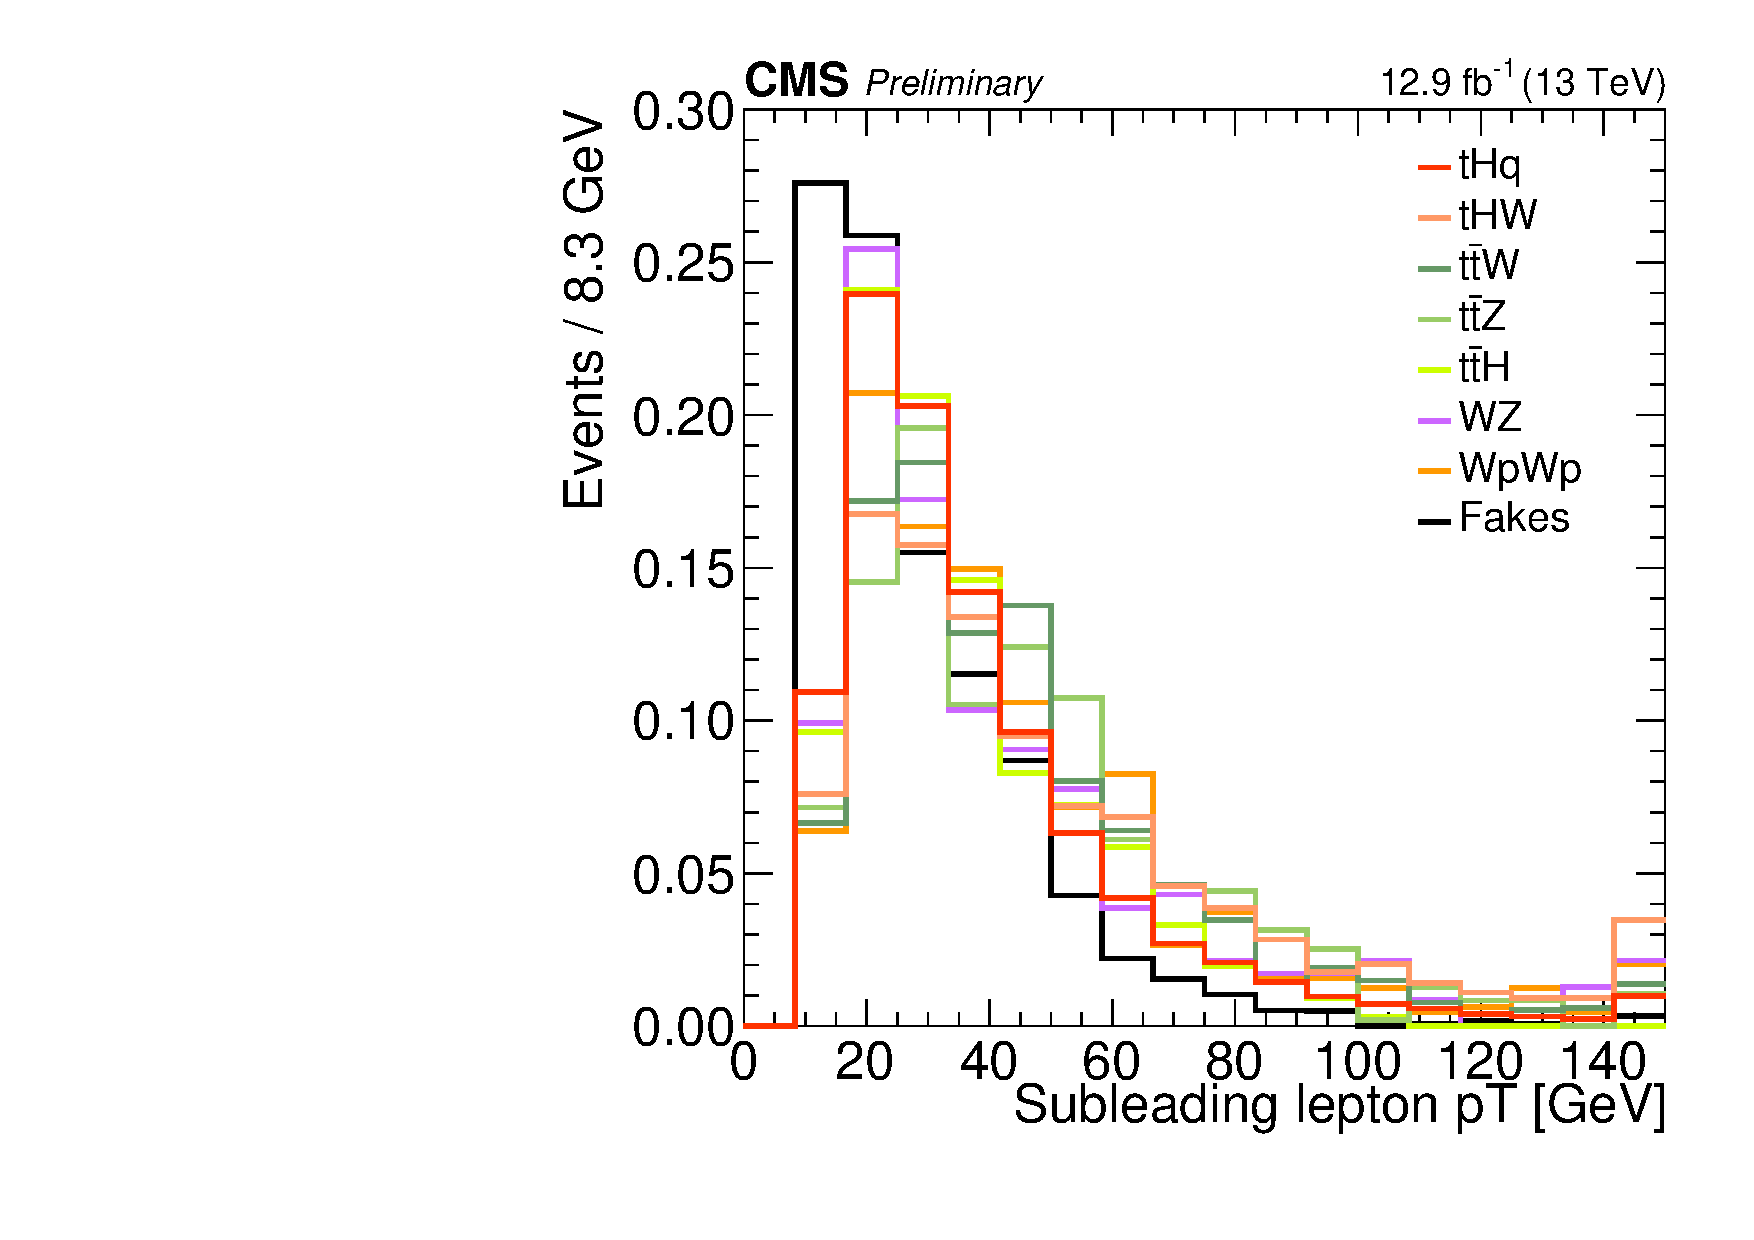
\includegraphics[width=0.32\textwidth]{Lep2Pt_mumu.pdf}
  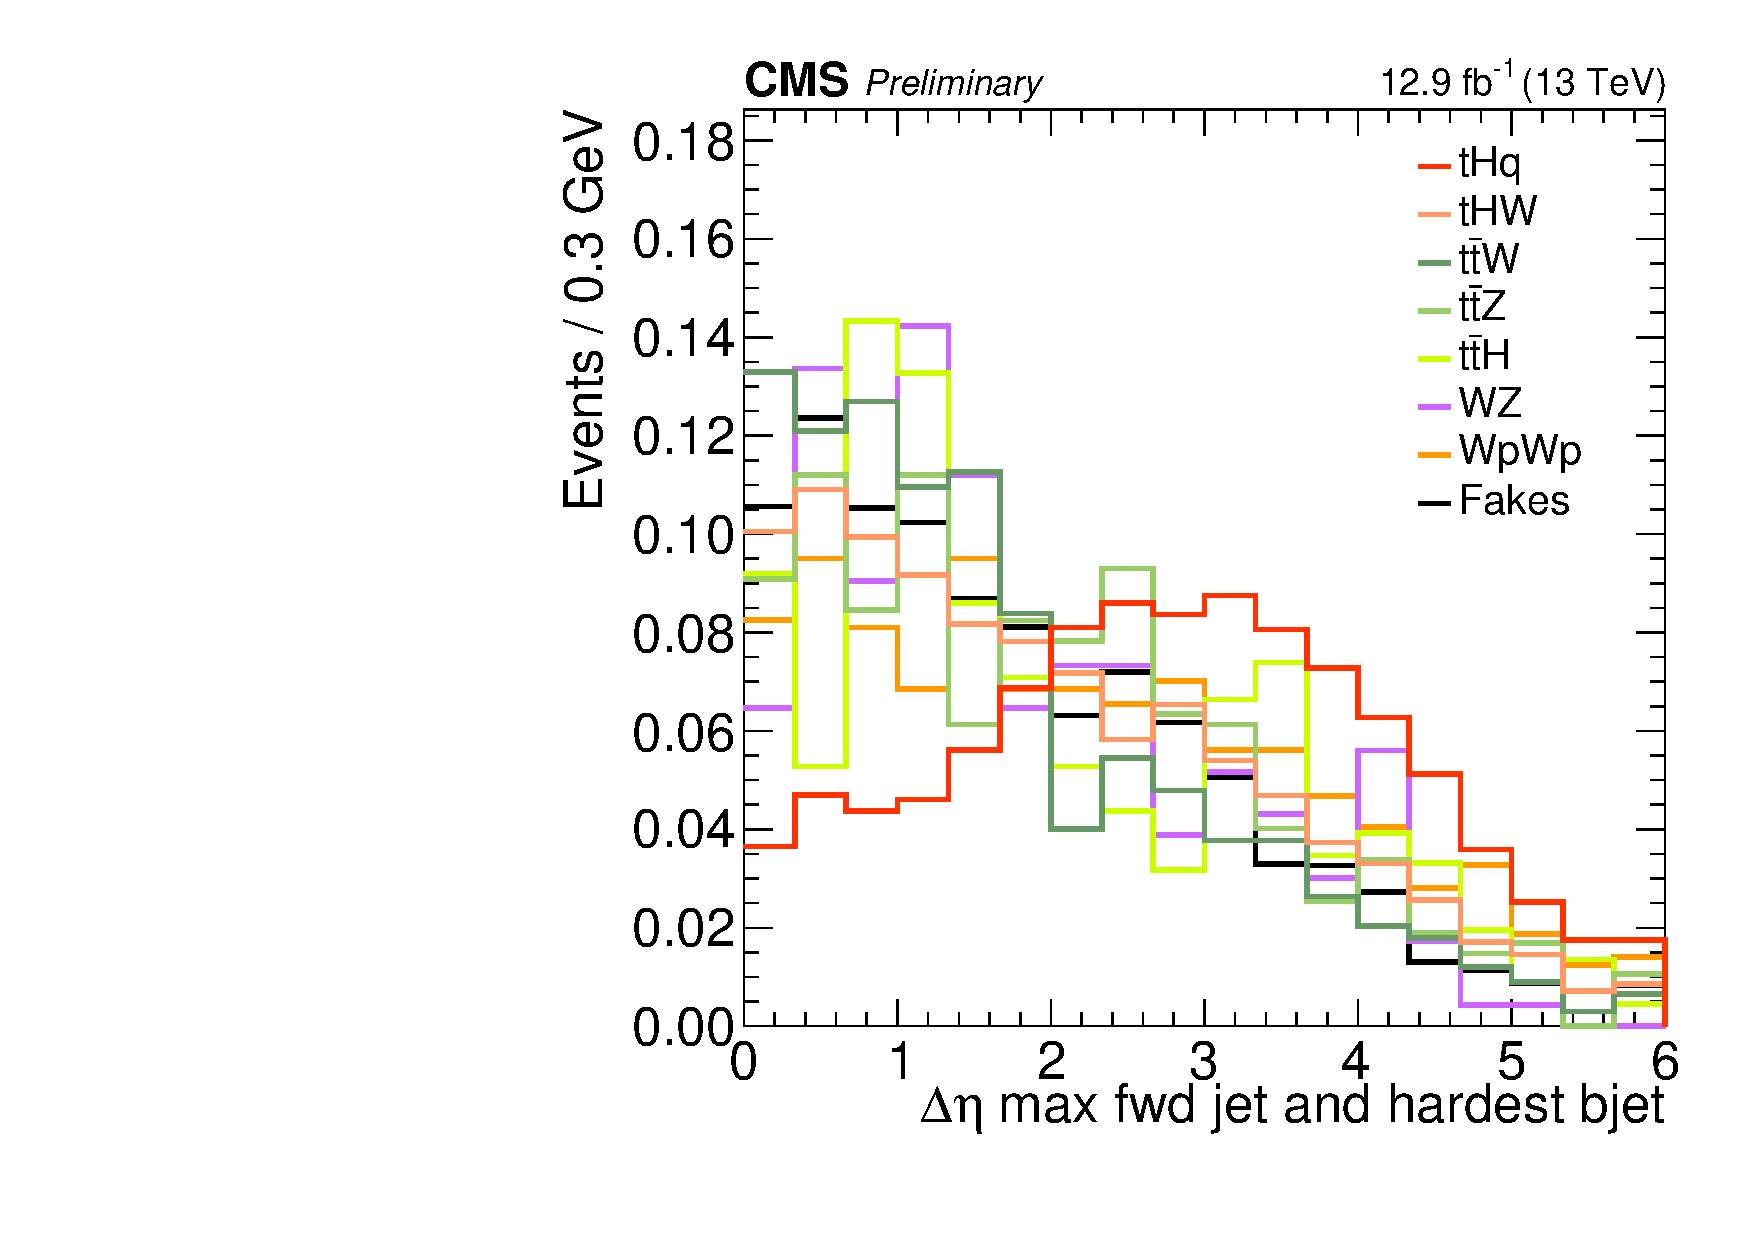
\includegraphics[width=0.32\textwidth]{dEtaFwdJetBJet_mumu.pdf}
  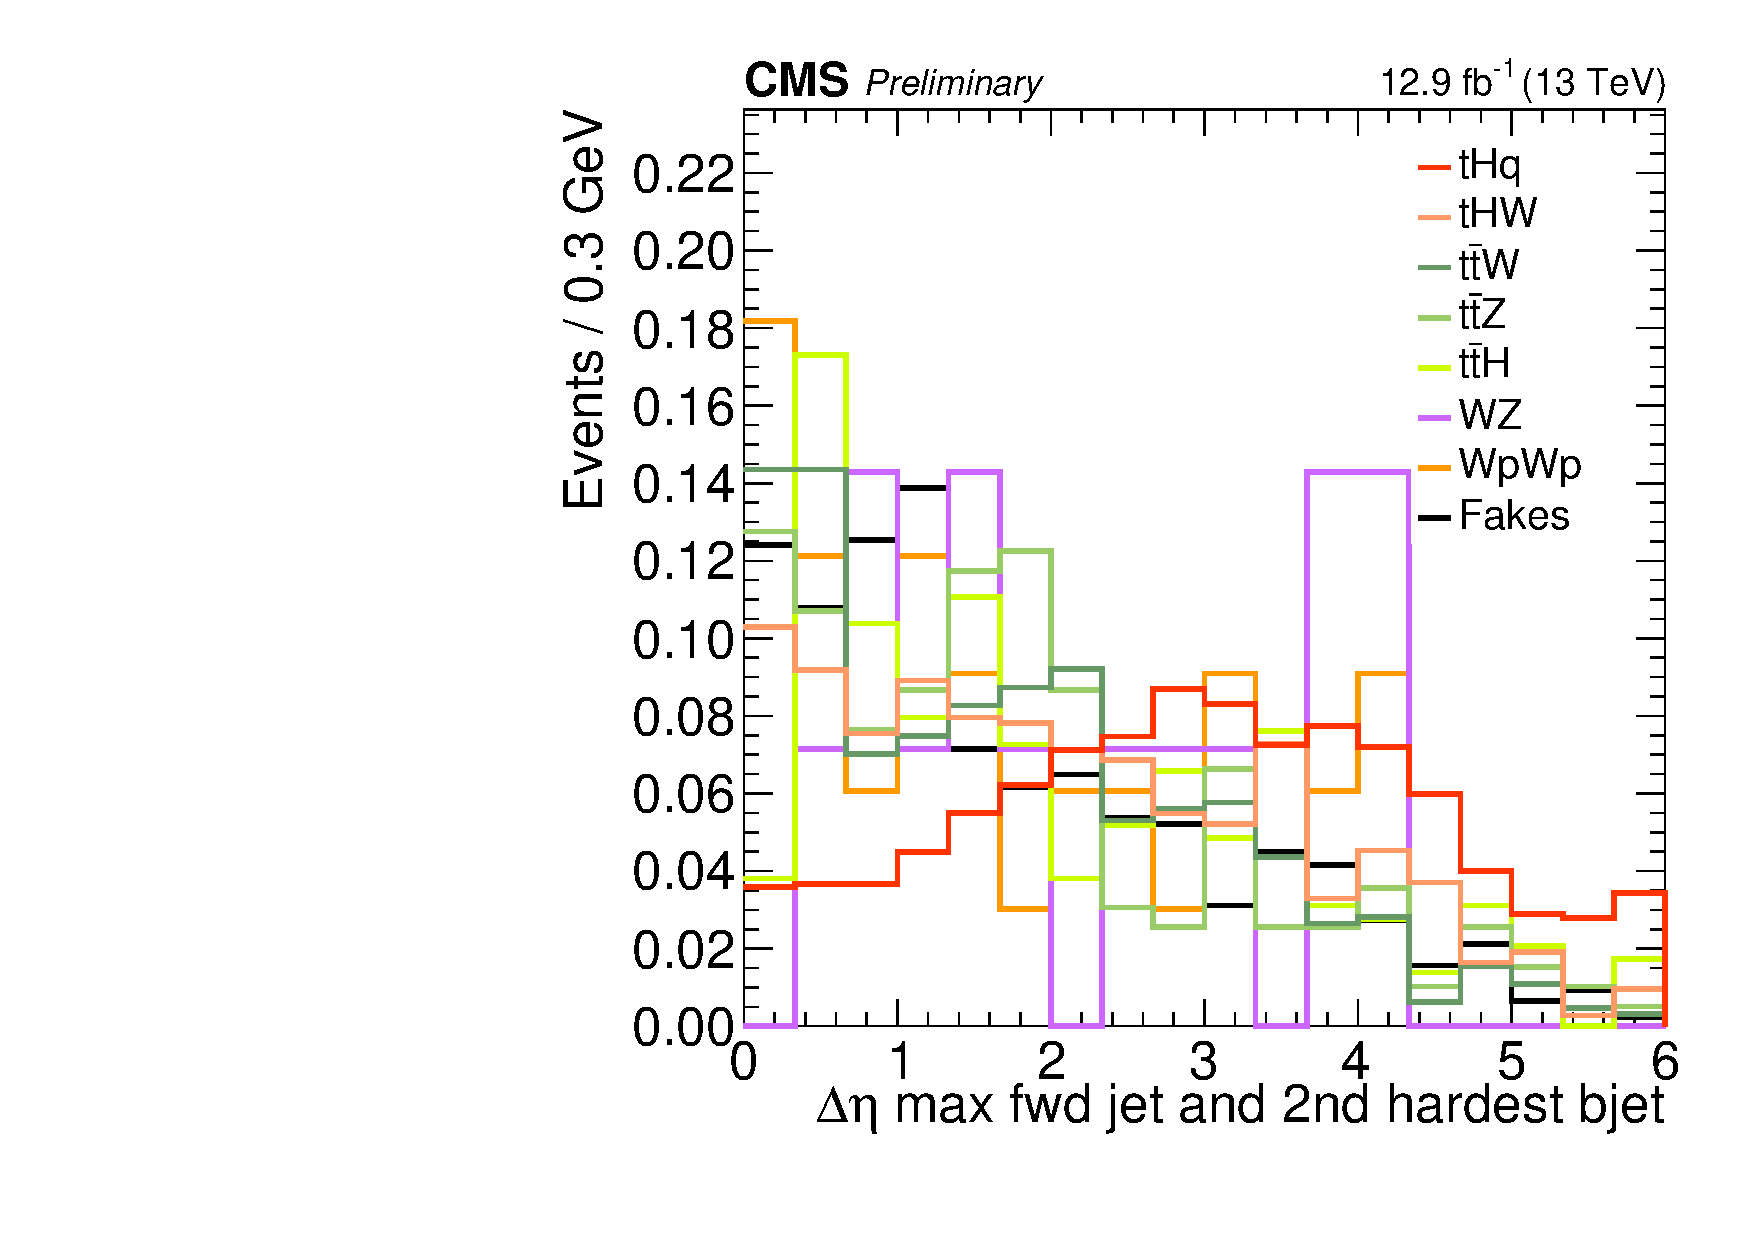
\includegraphics[width=0.32\textwidth]{dEtaFwdJet2BJet_mumu.pdf}\\
  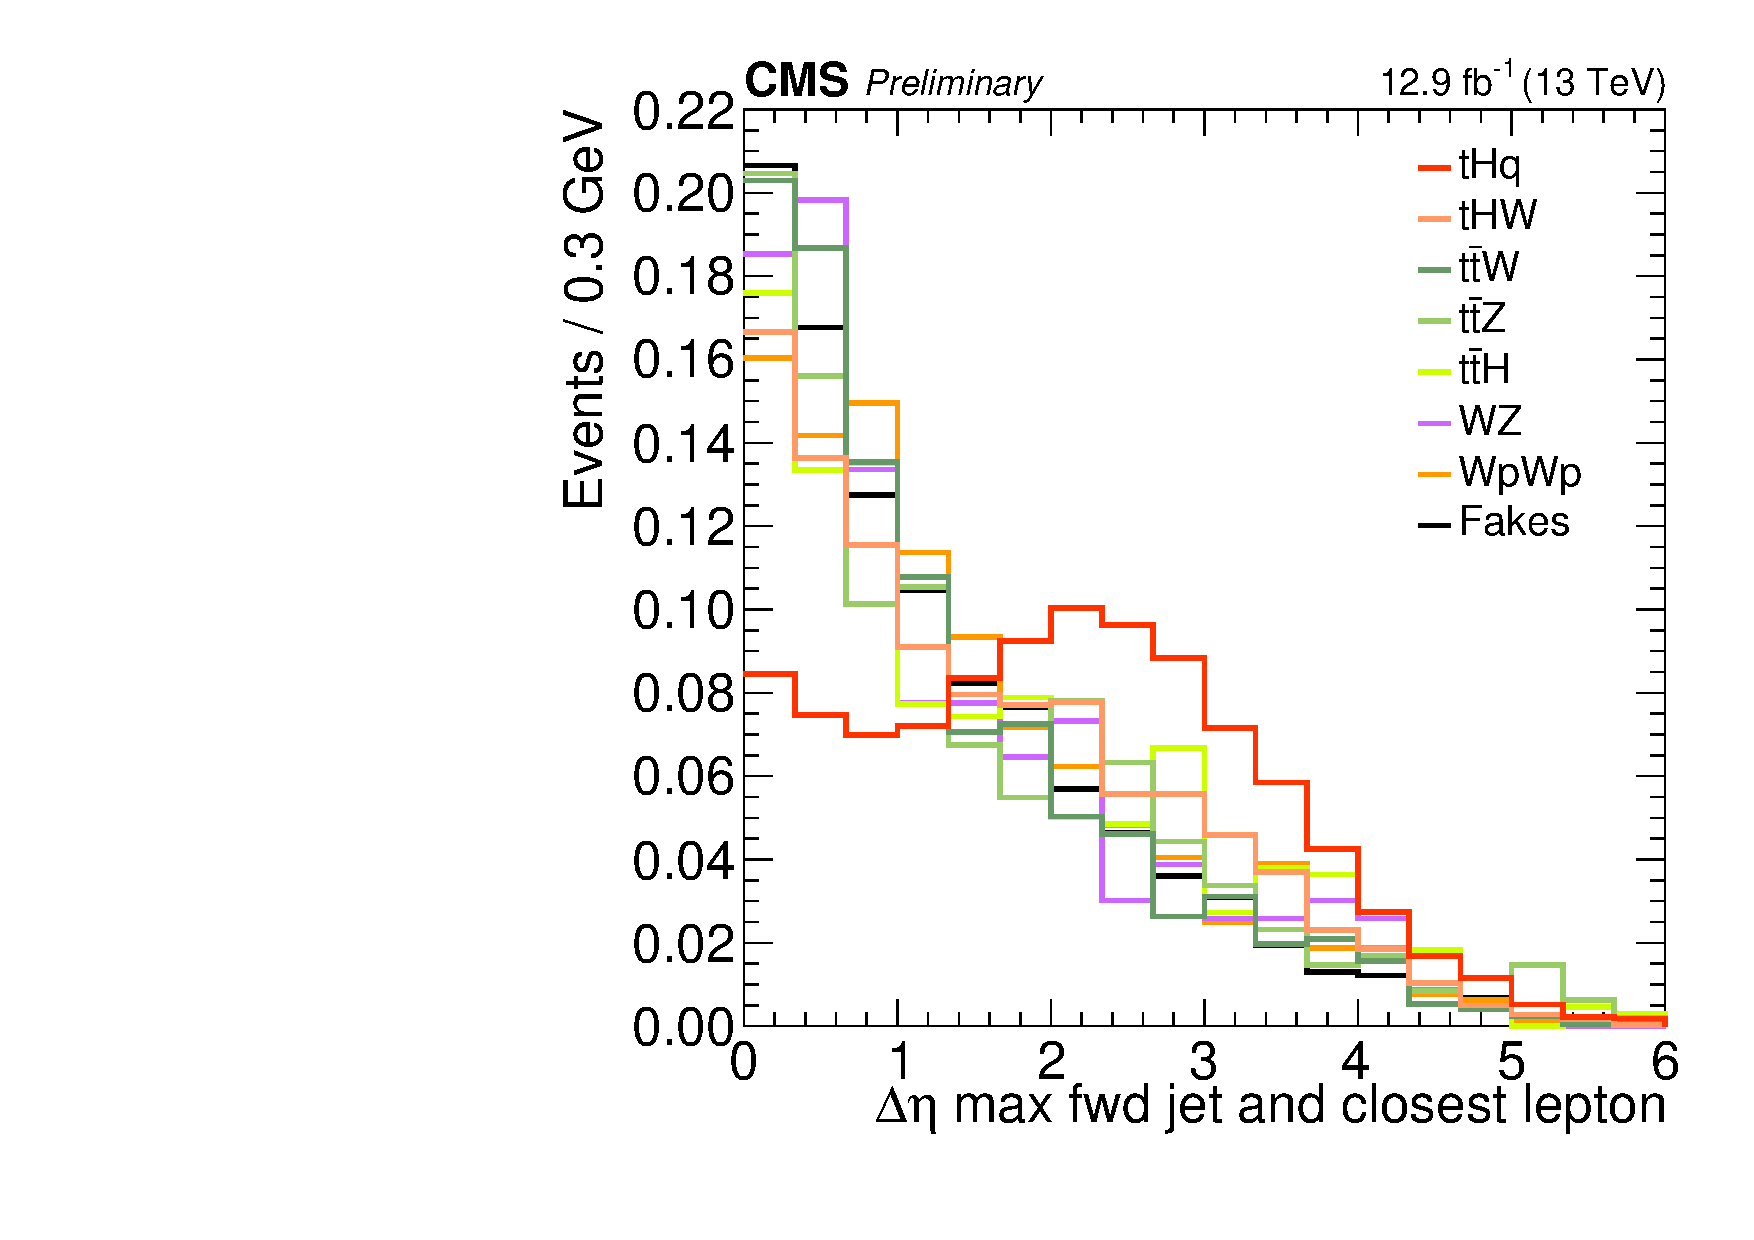
\includegraphics[width=0.32\textwidth]{dEtaFwdJetClosestLep_mumu.pdf}
  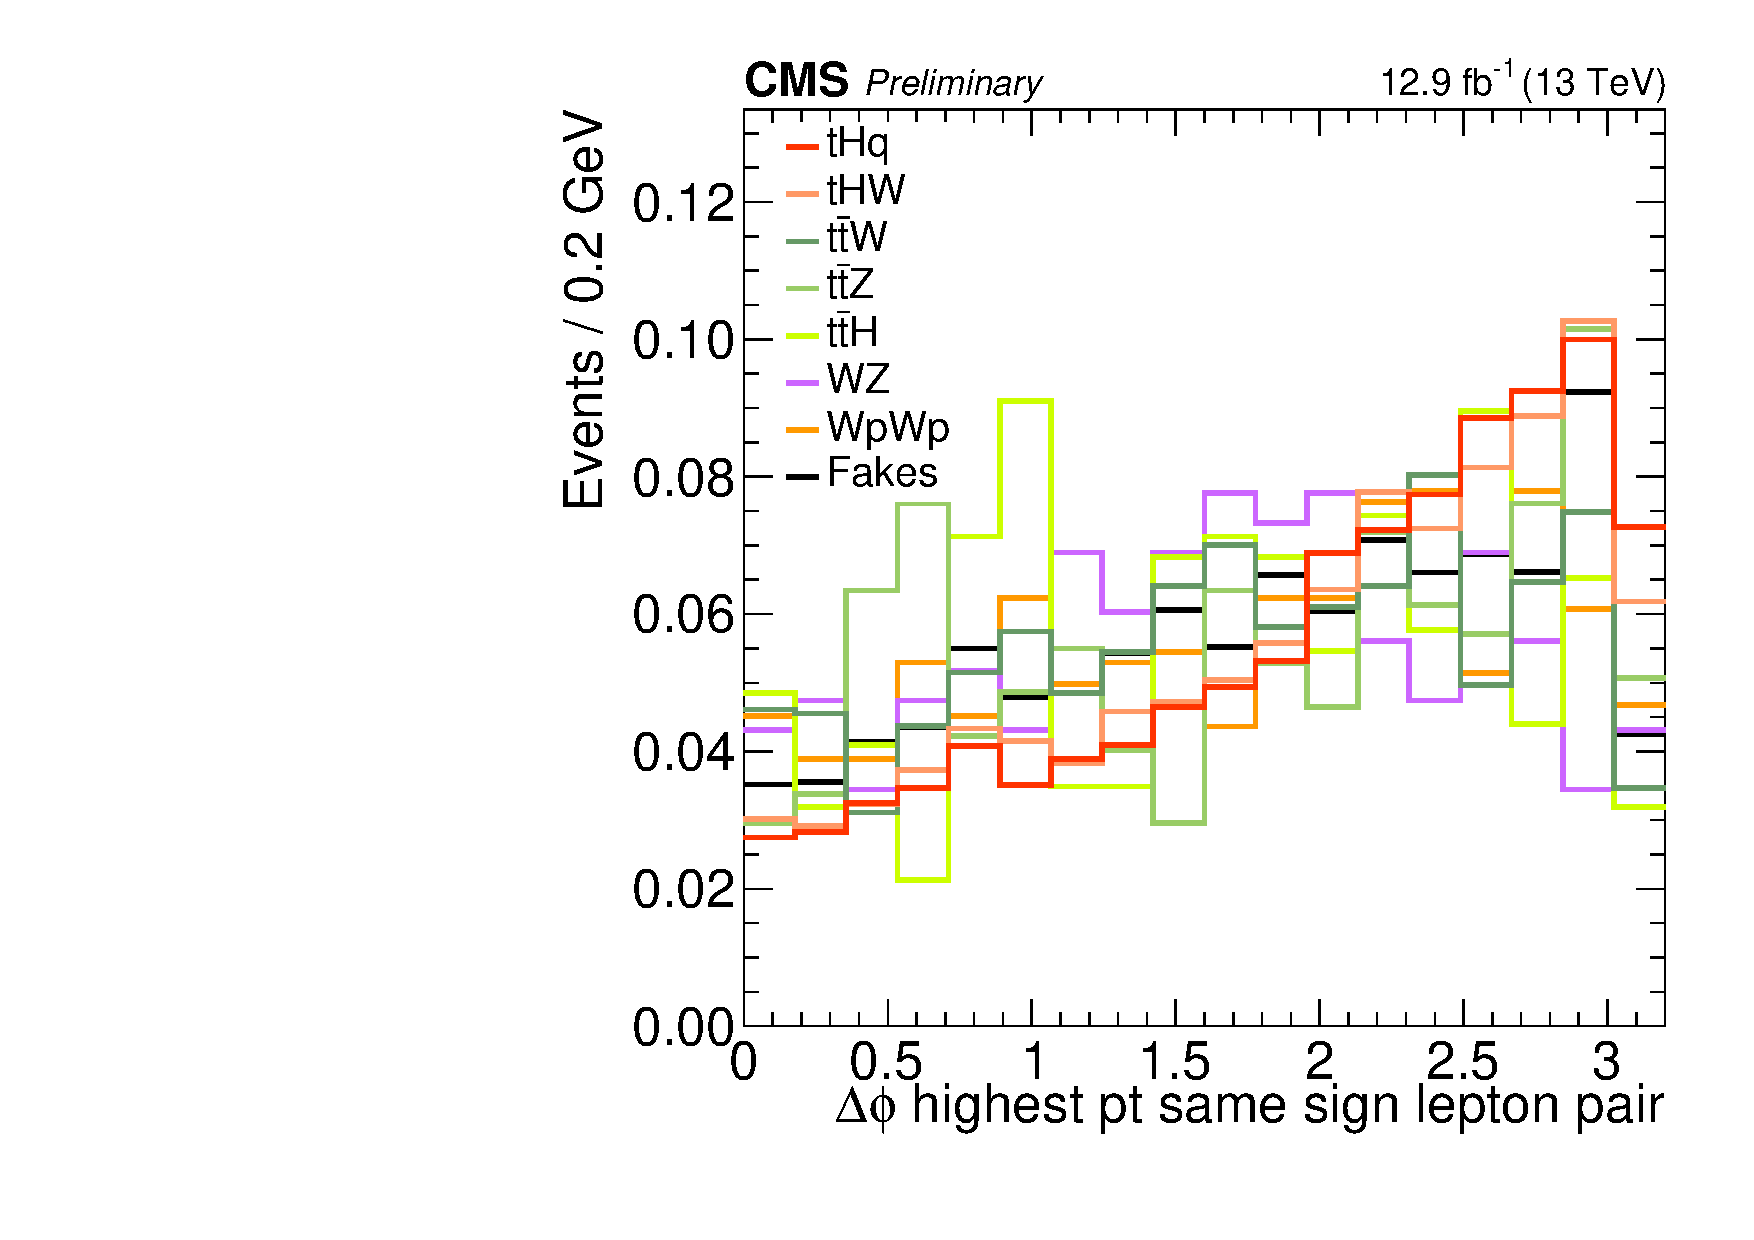
\includegraphics[width=0.32\textwidth]{dPhiHighestPtSSPair_mumu.pdf}
  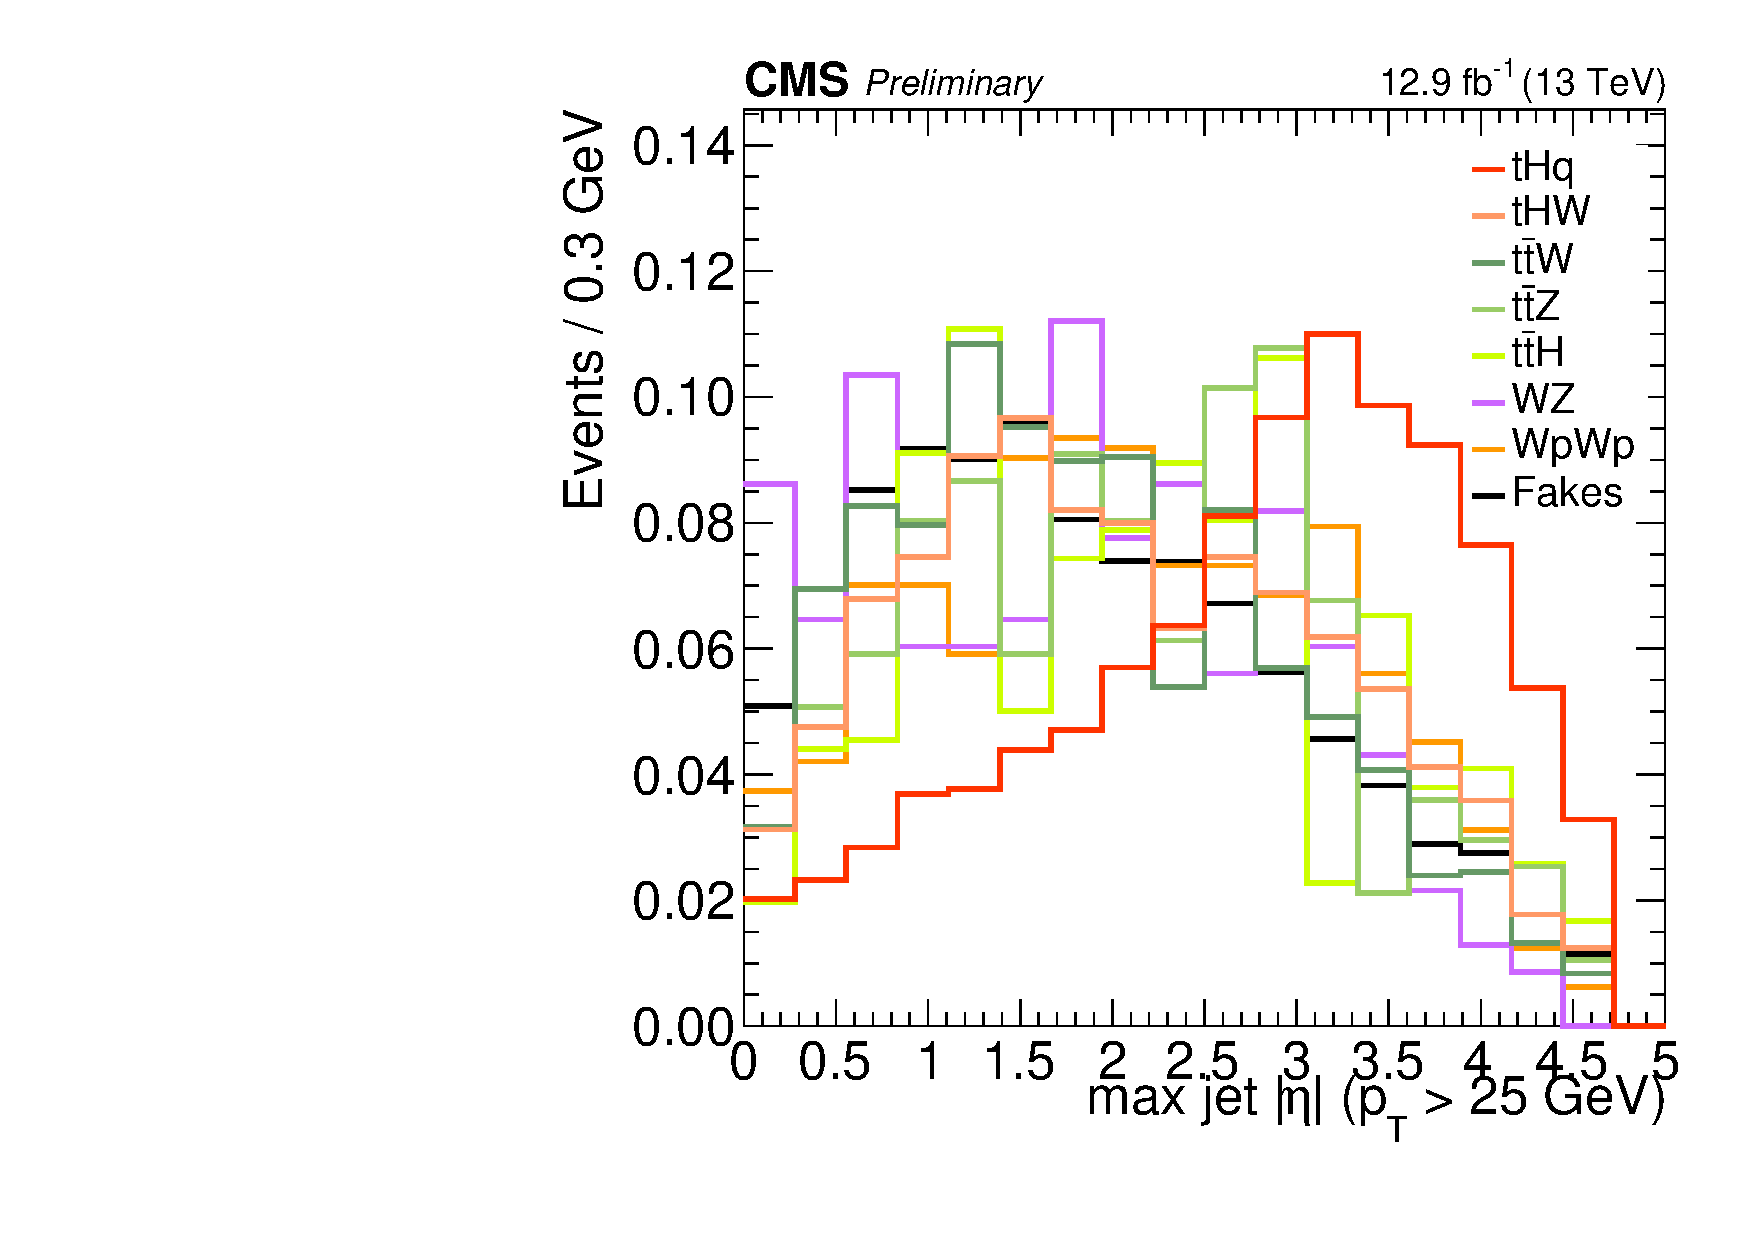
\includegraphics[width=0.32\textwidth]{maxEtaJet25_mumu.pdf}\\
  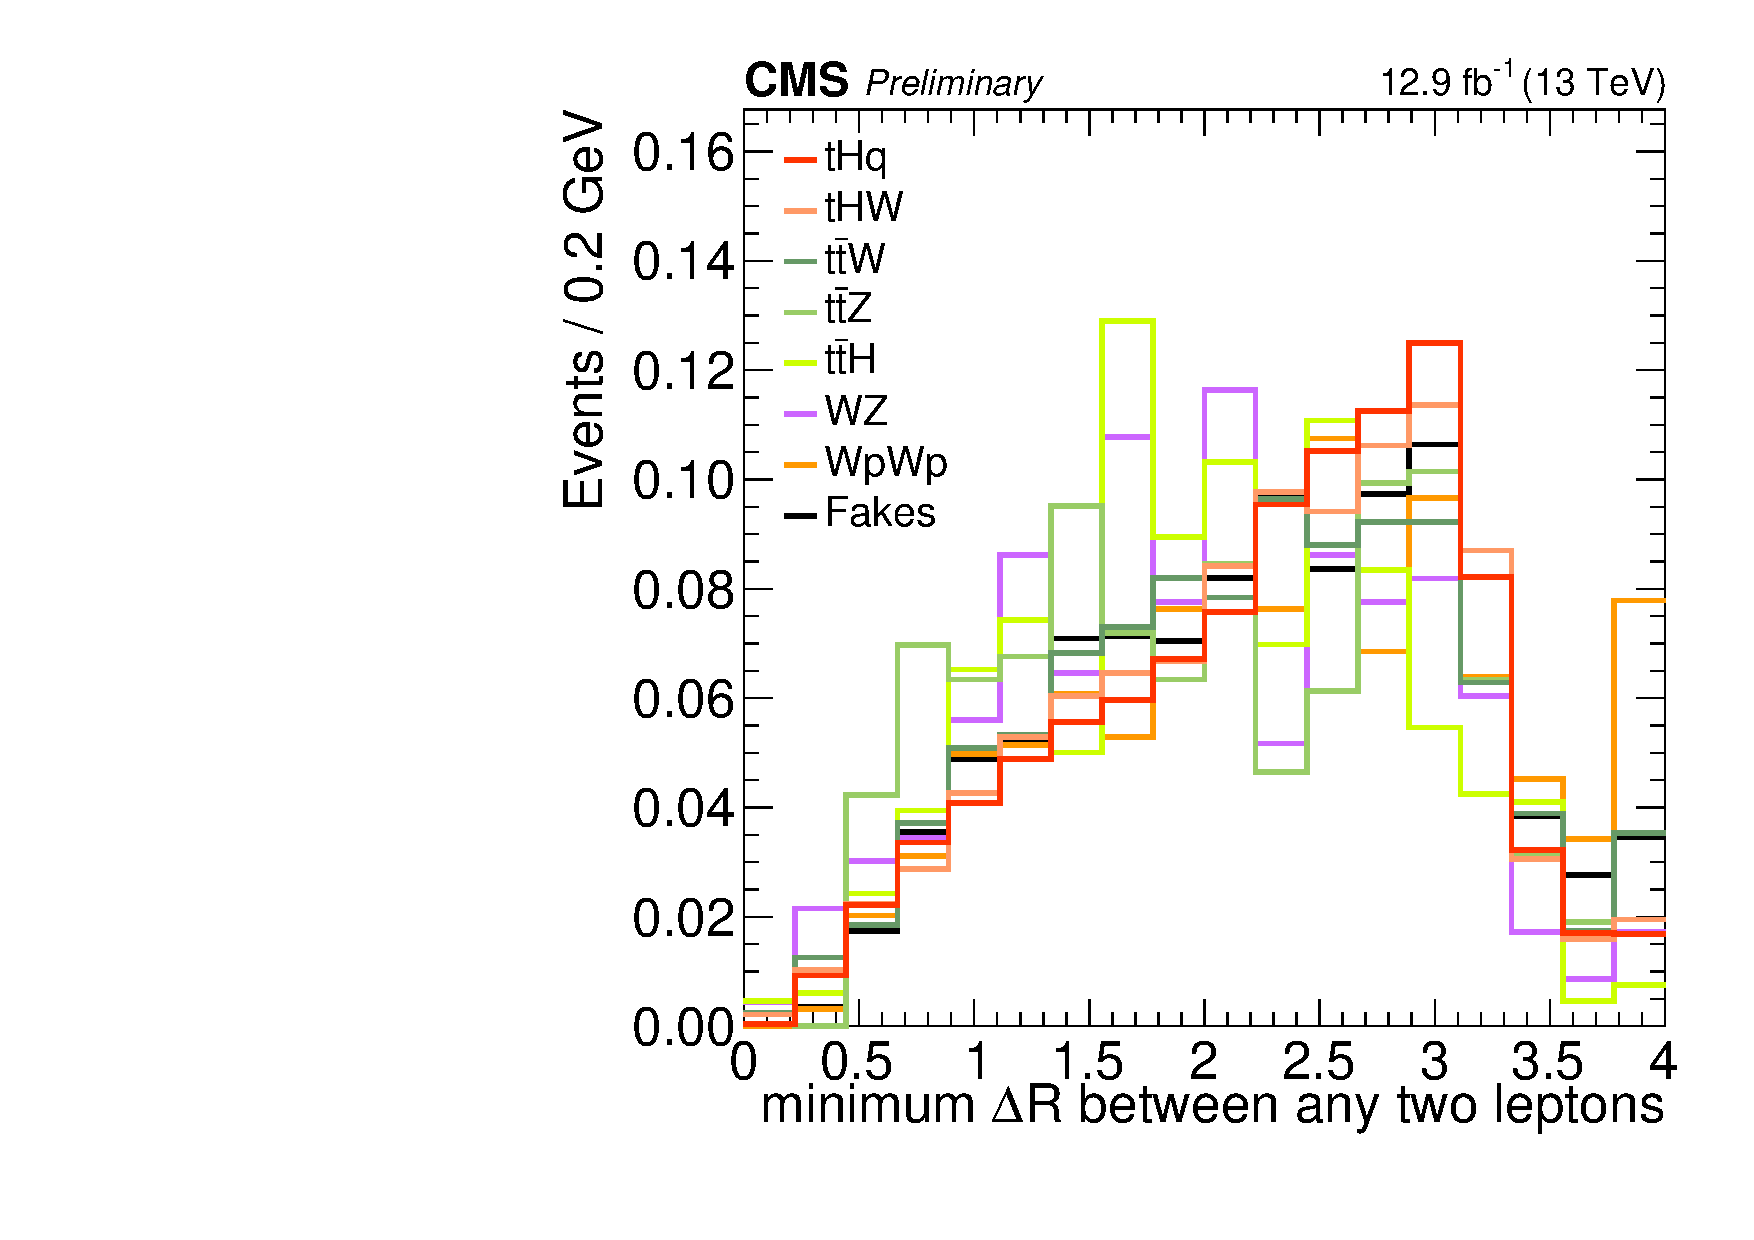
\includegraphics[width=0.32\textwidth]{minDRll_mumu.pdf}
  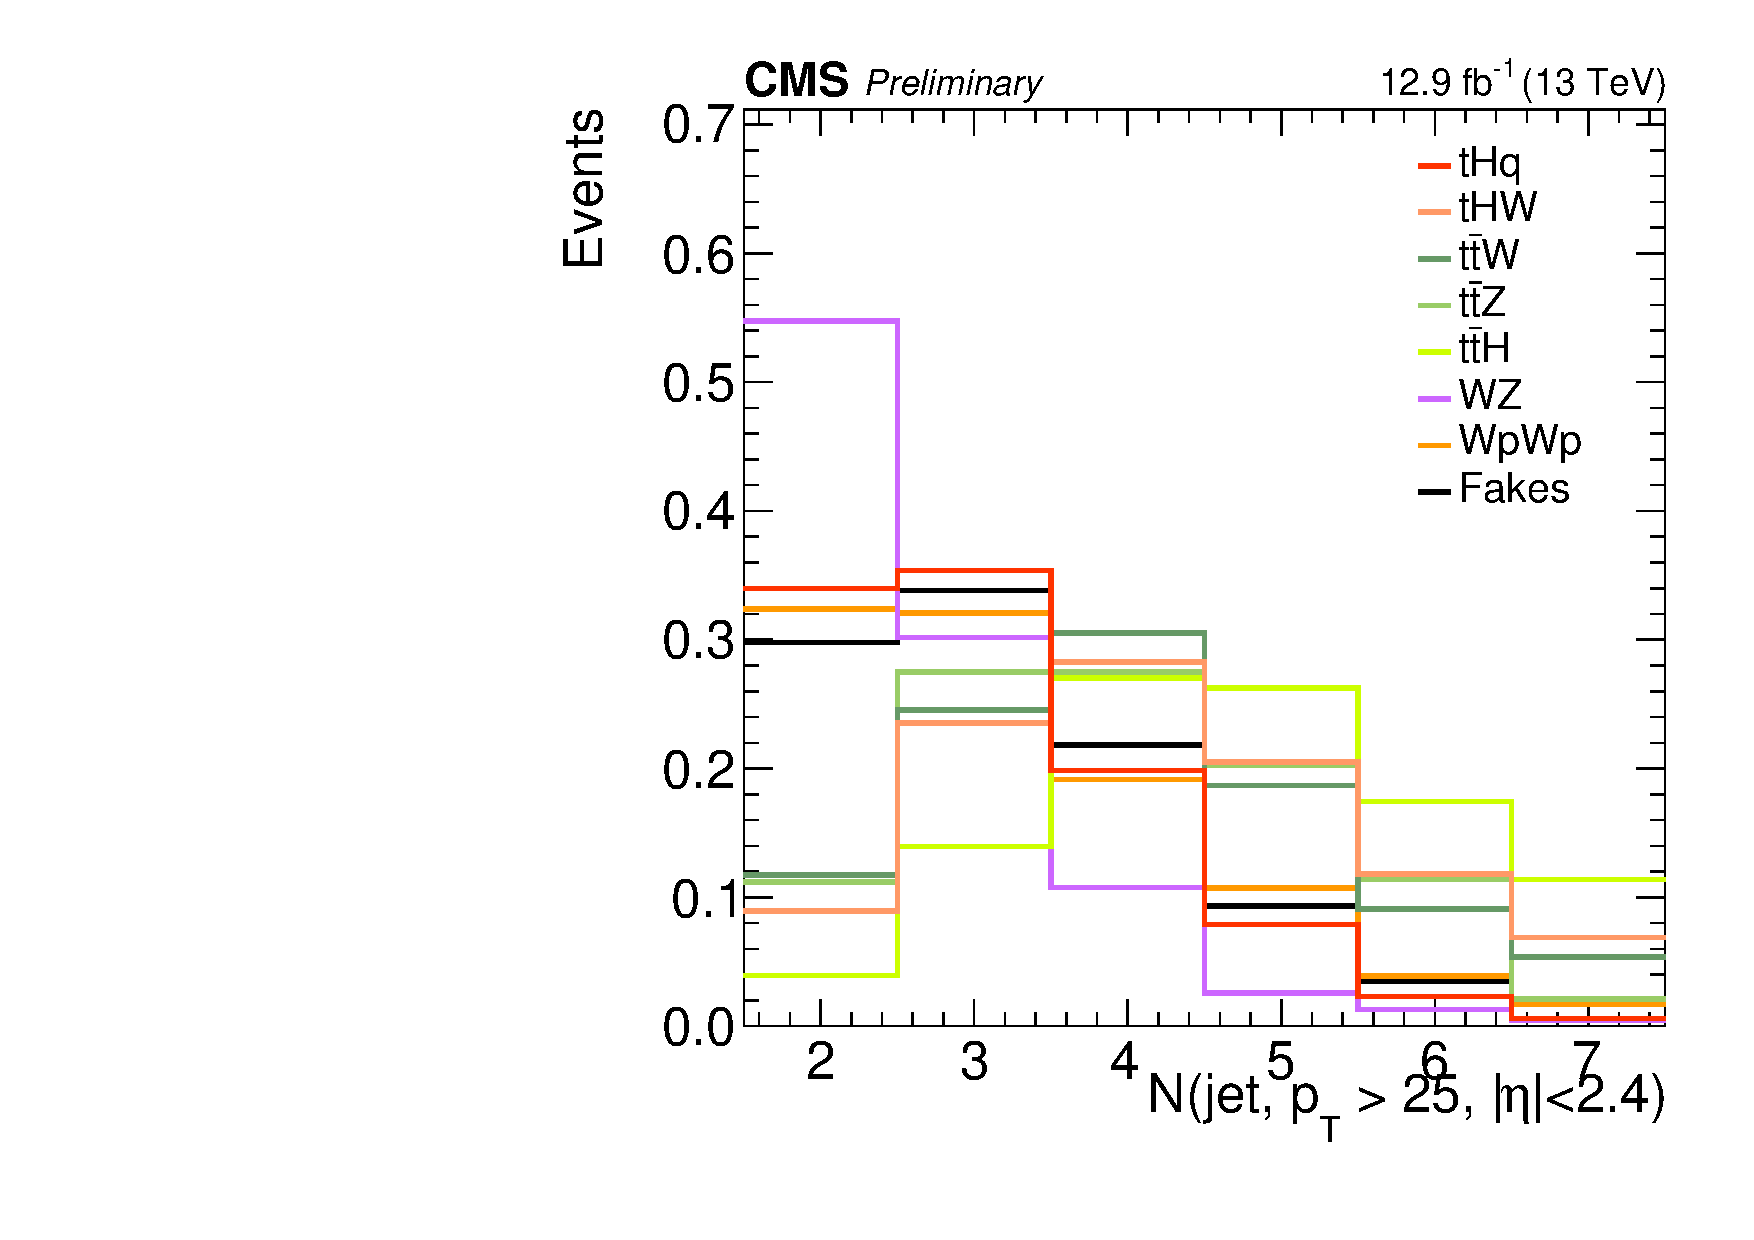
\includegraphics[width=0.32\textwidth]{nJet25_mumu.pdf}
  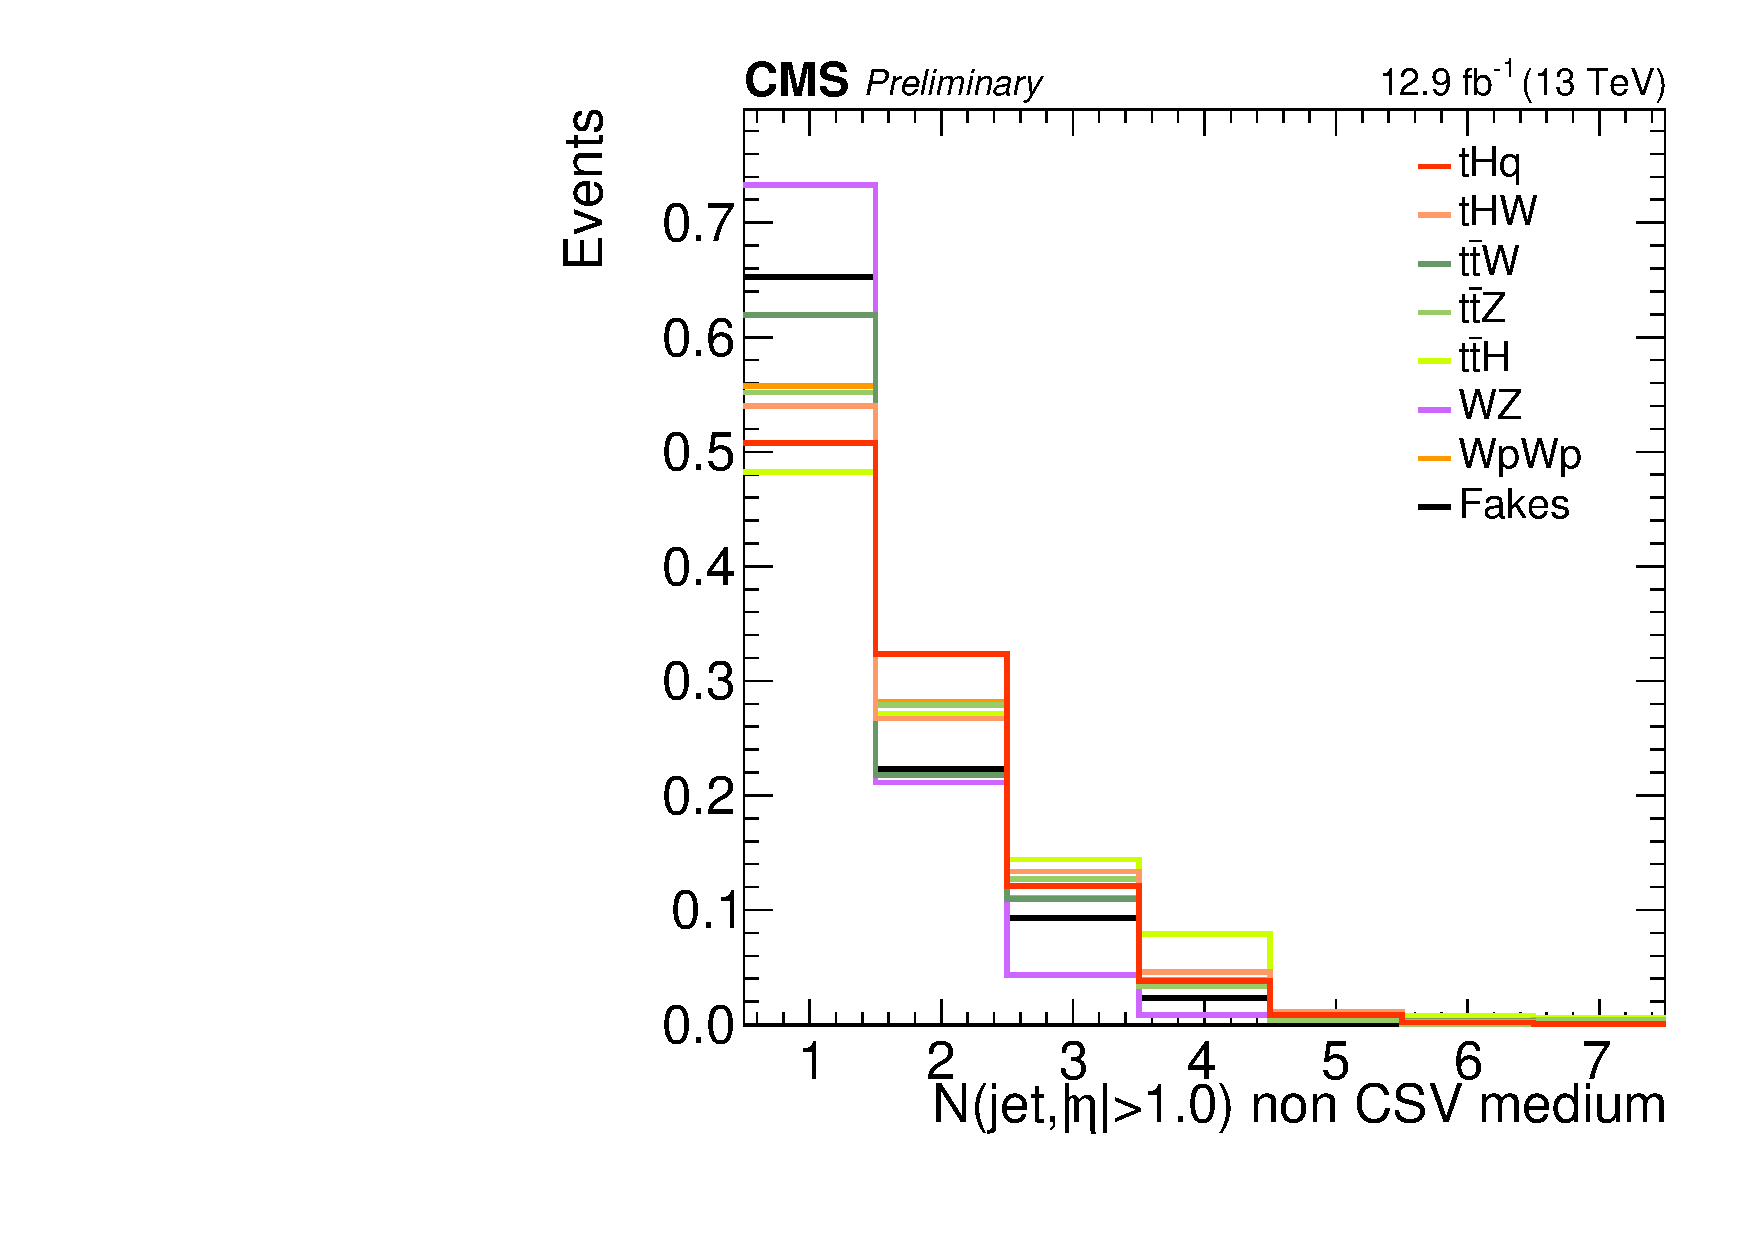
\includegraphics[width=0.32\textwidth]{nJetEta1_mumu.pdf}\\
  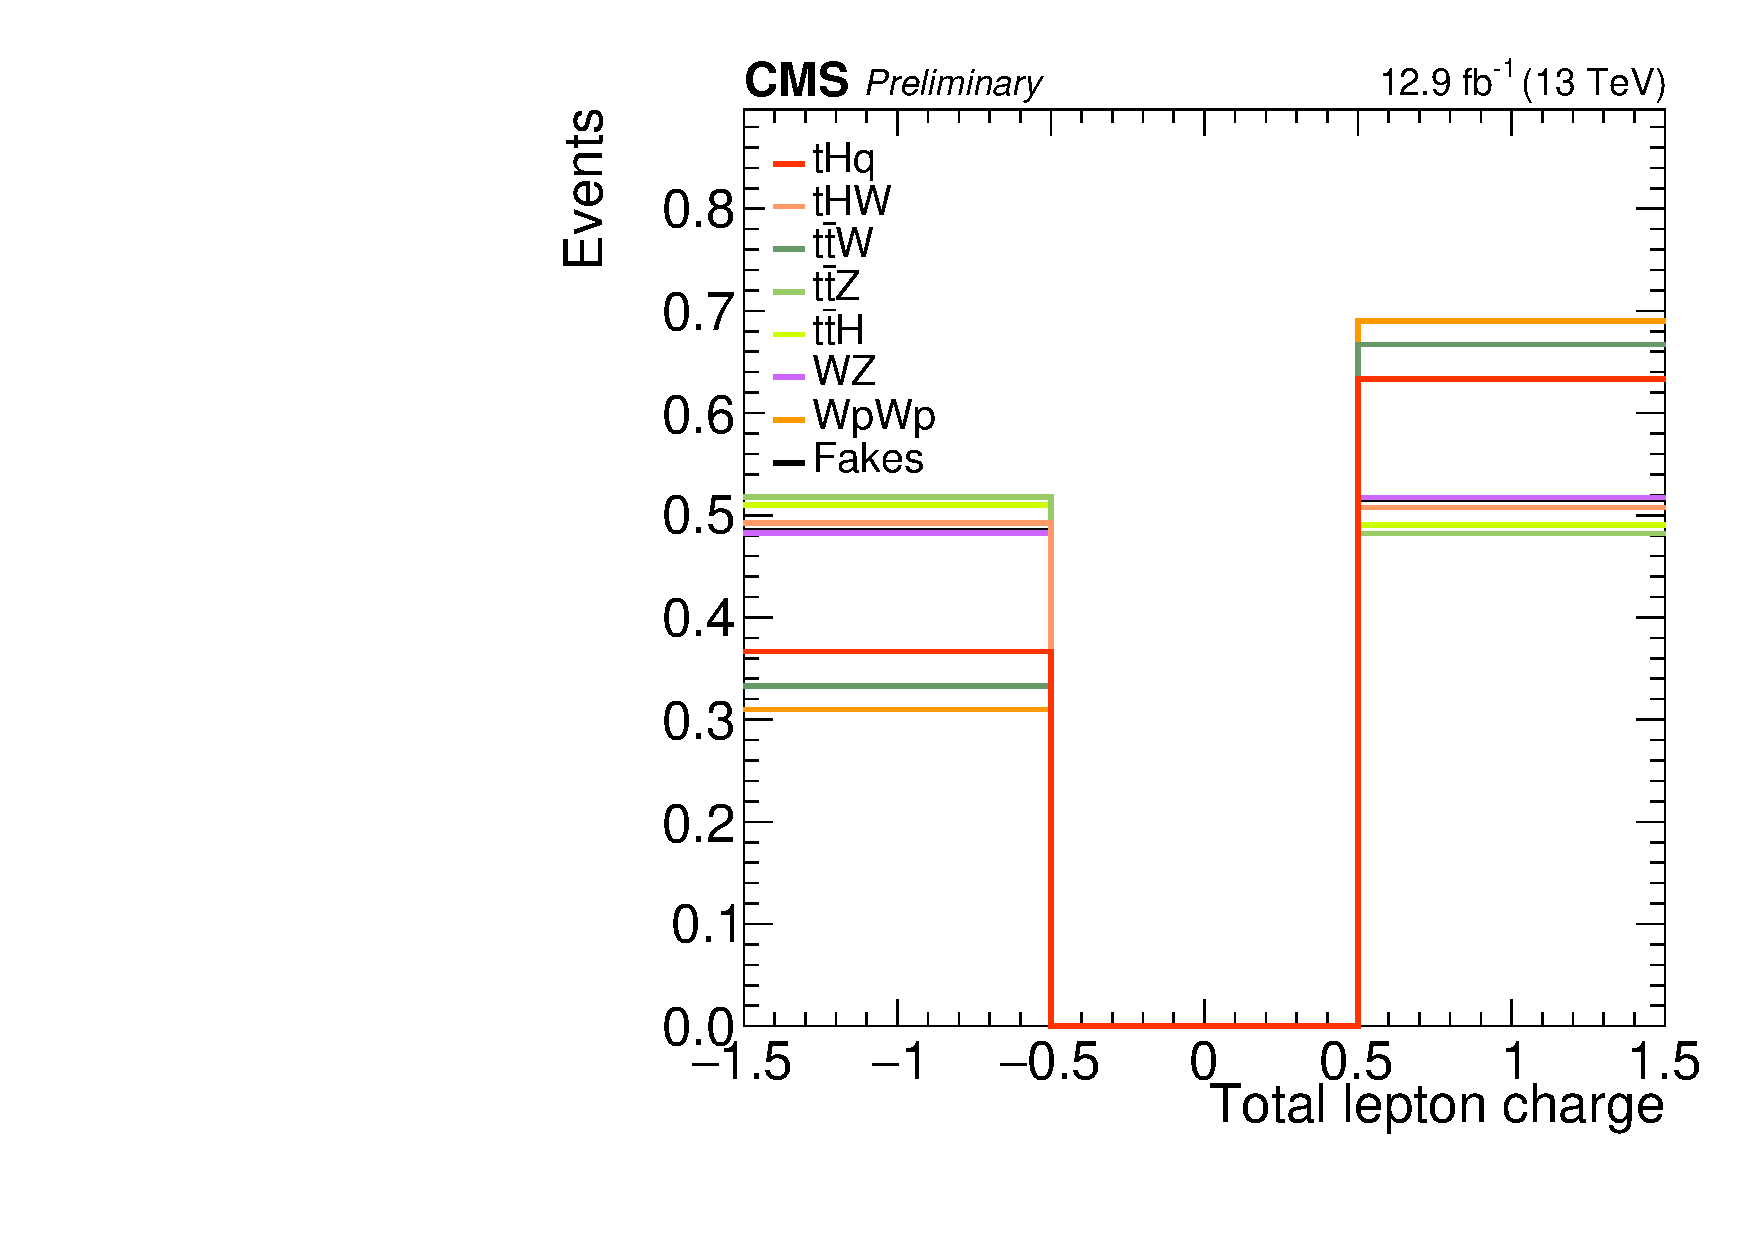
\includegraphics[width=0.32\textwidth]{totCharge_mumu.pdf}
  \caption{Distributions of input variables to the BDT for signal discrimination, two lepton same sign channel.}
  \label{fig:input_vars_2lss}
\end{figure}  
\newpage
\section{Input variables distributions from BDTG classifiers}

\begin{figure} [!h]
  \centering
  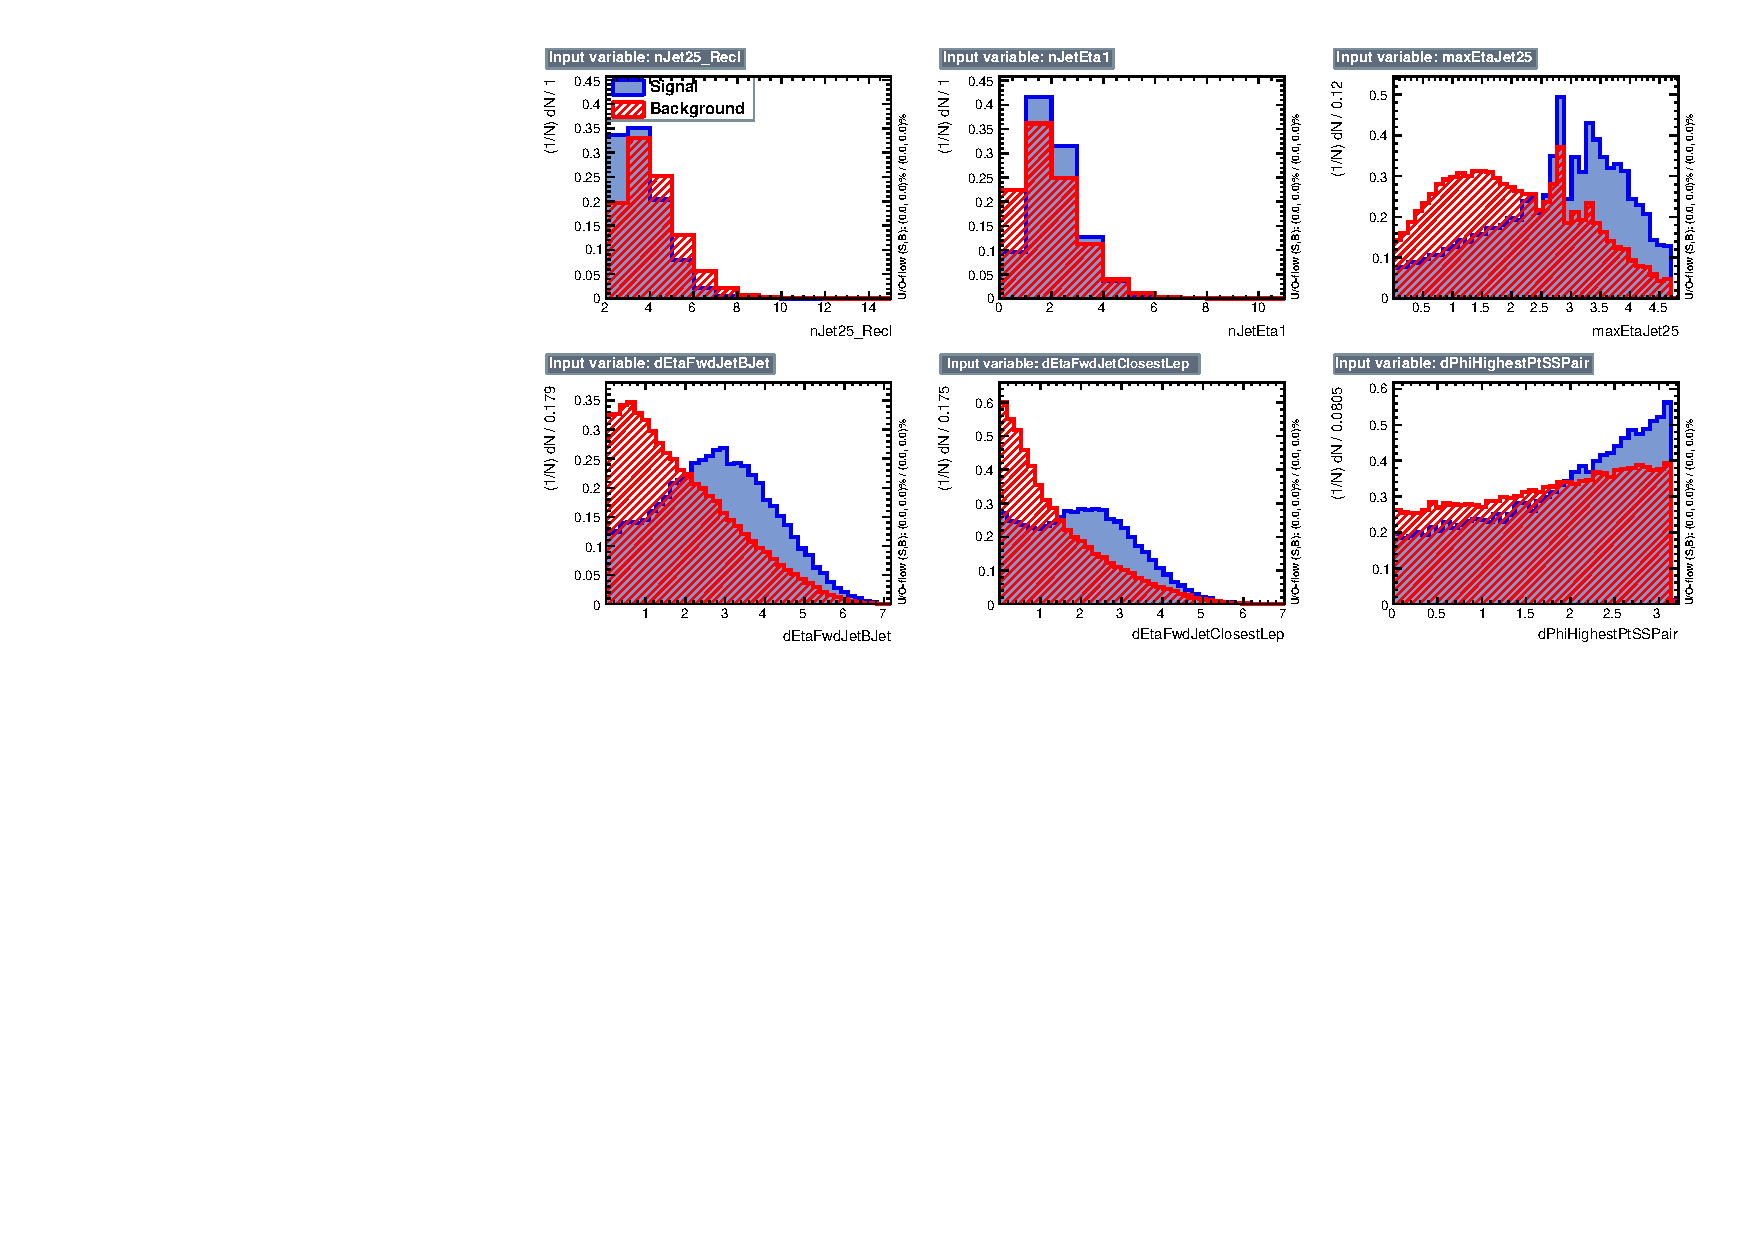
\includegraphics[width=\textwidth]{6var_tt.pdf}
  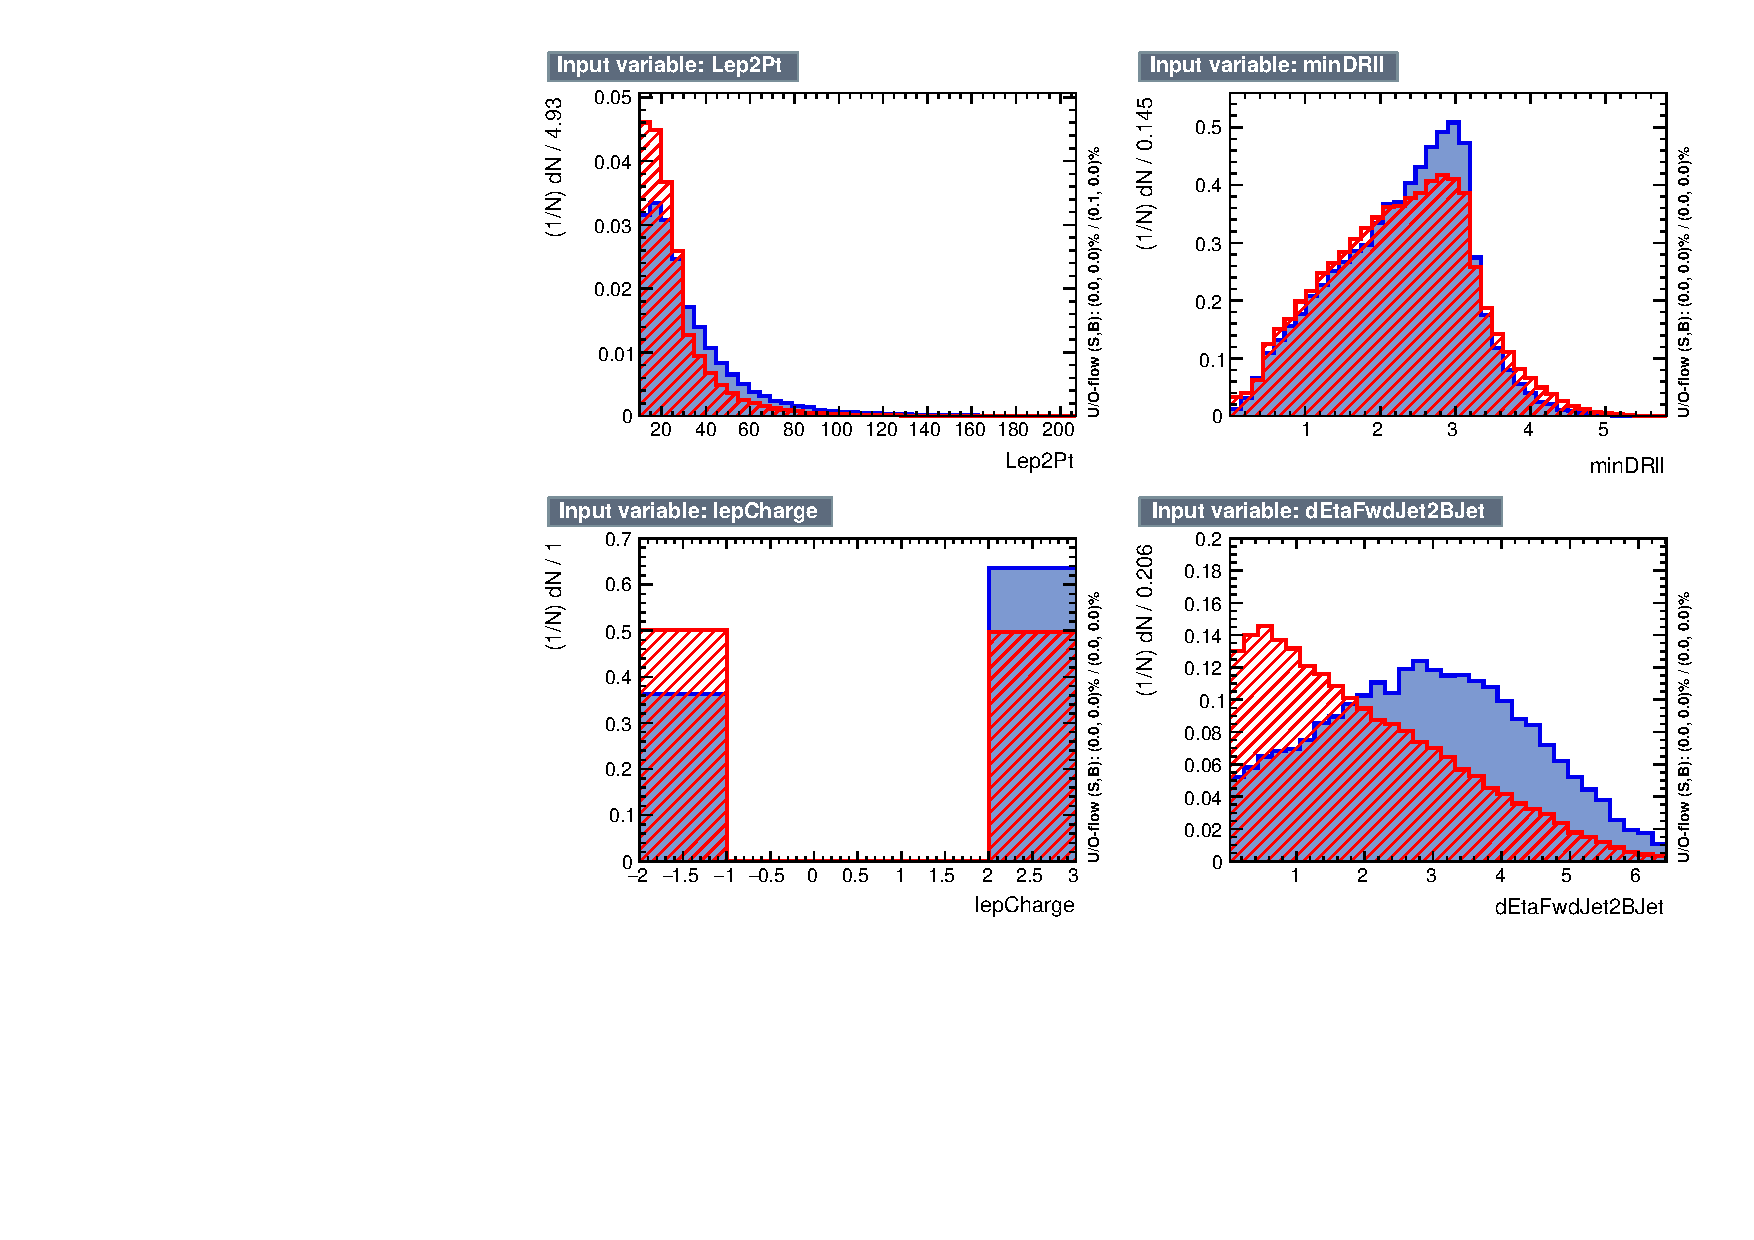
\includegraphics[width=0.66\textwidth]{4var_tt.pdf}
  \caption[BDT input variables. Discrimination against \ttbar\ in $2lss$ channel.]{BDT input variables as seen by BDTG classifier for the $2lss$ channel, \tHq signal (blue) discriminated against \ttbar\ background (red).}
  \label{mva_input_2lss_tt}
\end{figure}

\begin{figure} [!h]
  \centering
  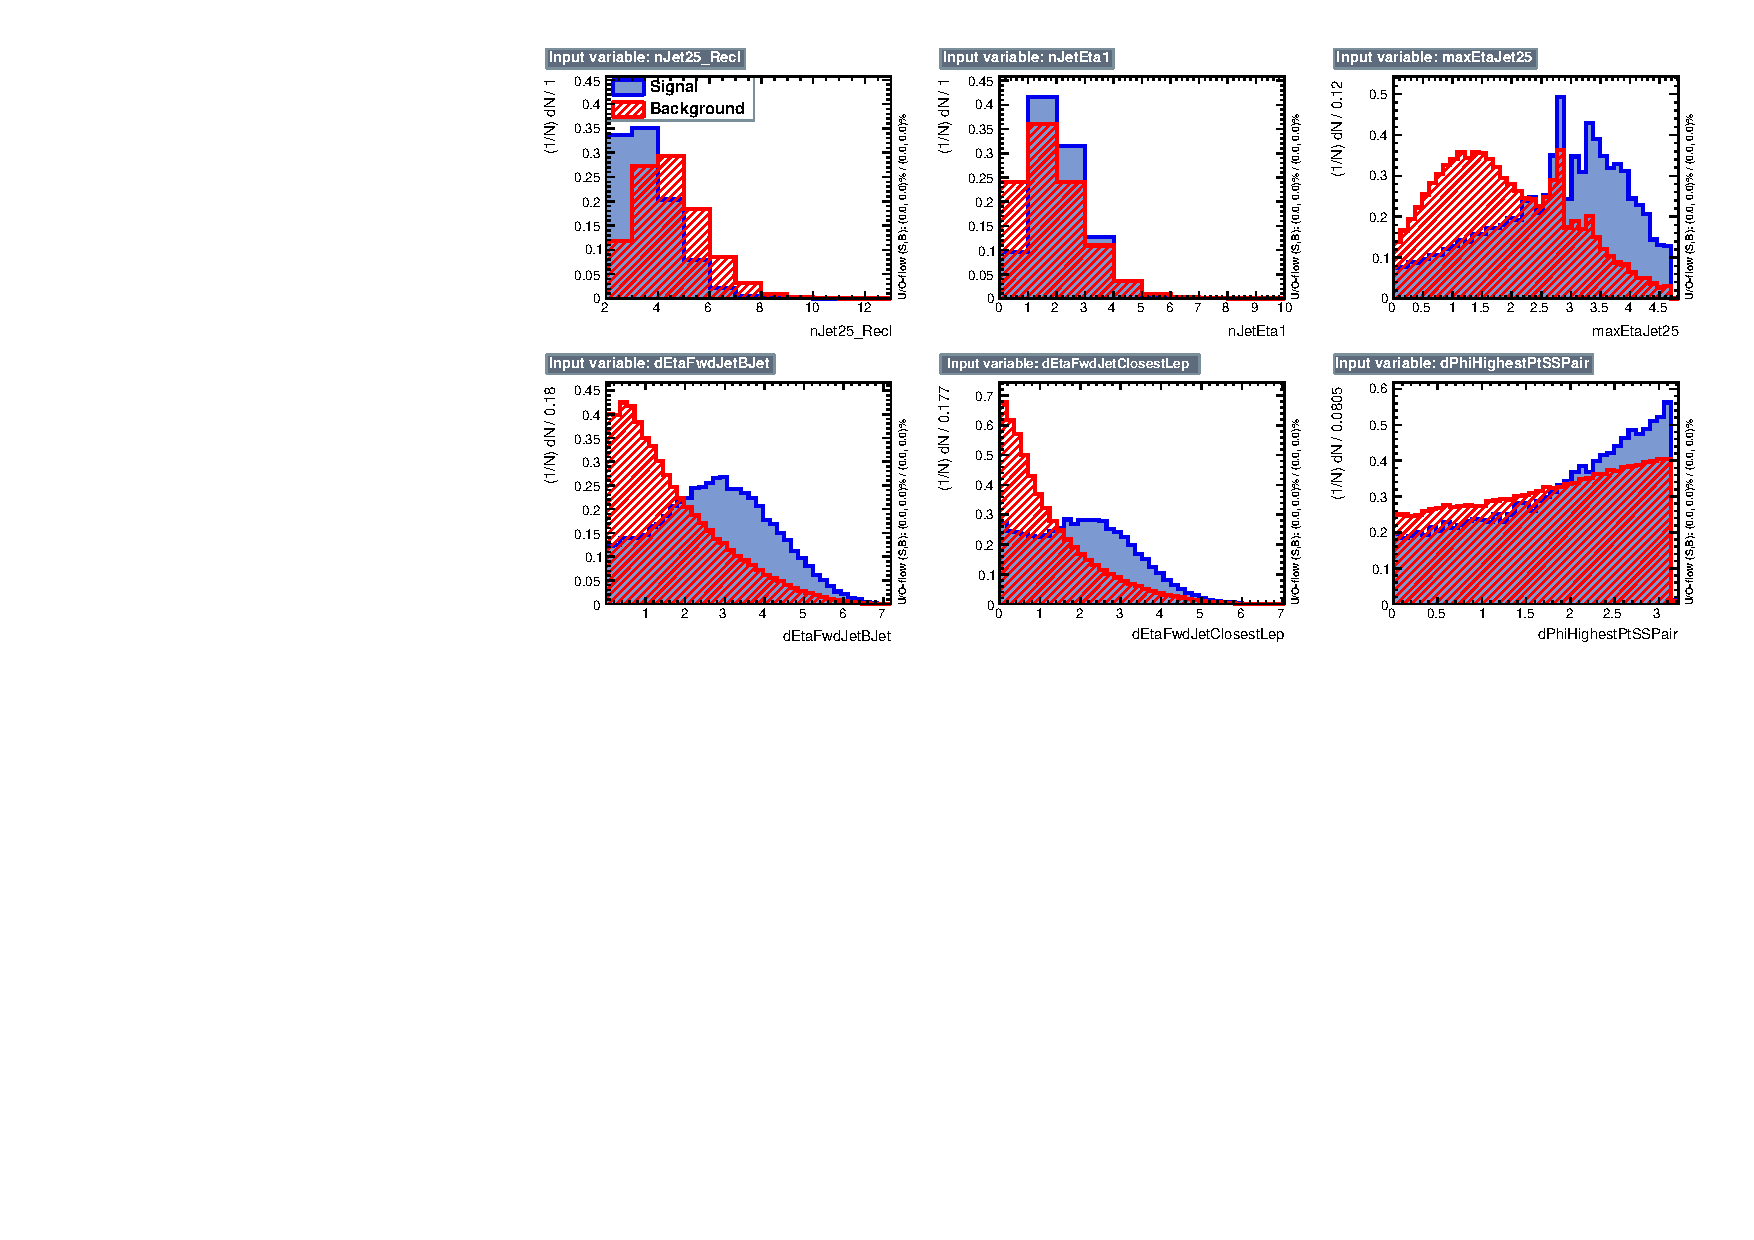
\includegraphics[width=\textwidth]{6var_ttv.pdf}
  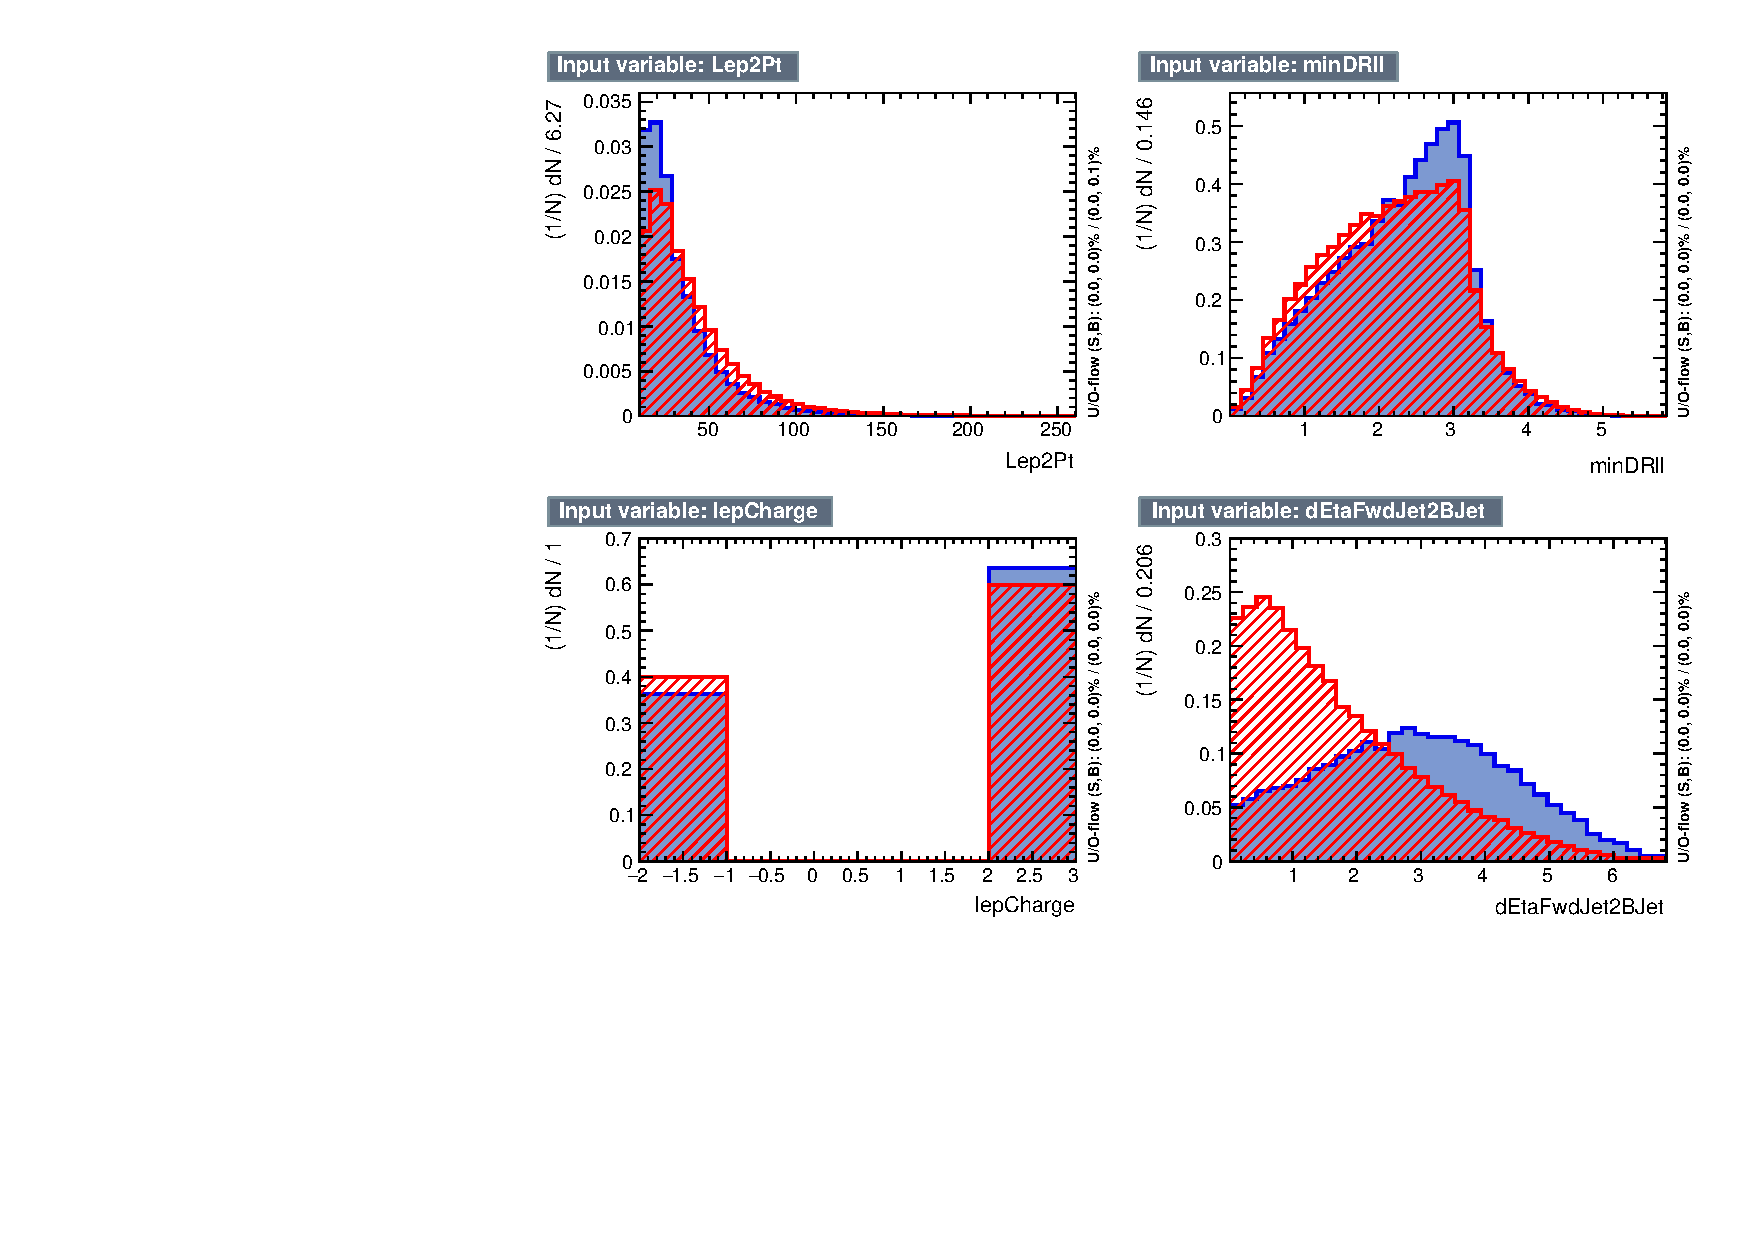
\includegraphics[width=0.66\textwidth]{4var_ttv.pdf}
  \caption[BDT input variables. Discrimination against \ttV\ in $2lss$ channel.]{BDT input variables as seen by BDTG classifier for the $2lss$ channel, \tHq signal(blue) discriminated against \ttV\ background (red).}
  \label{mva_input_2lss_ttv}
\end{figure}

\begin{figure} [!h]
  \centering
  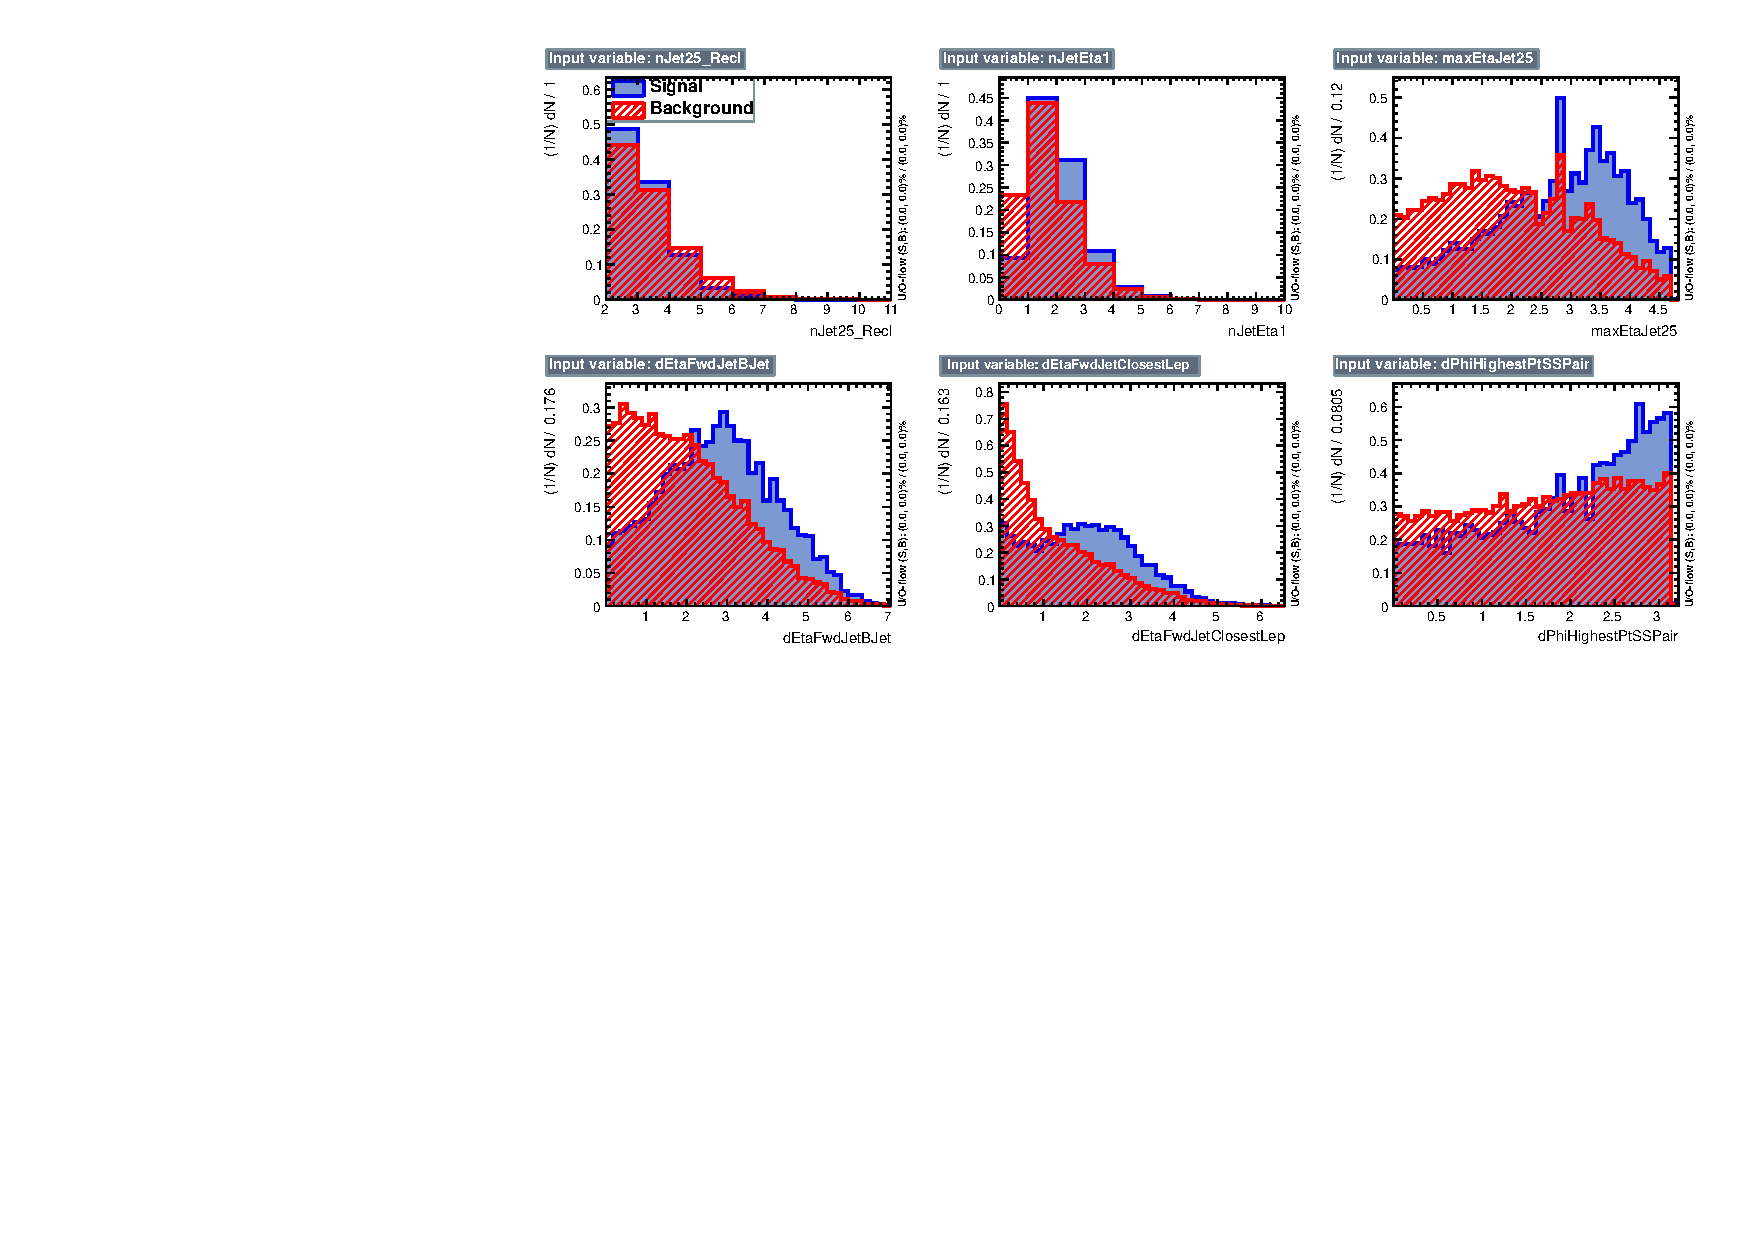
\includegraphics[width=\textwidth]{mva_input1_tt.pdf}
  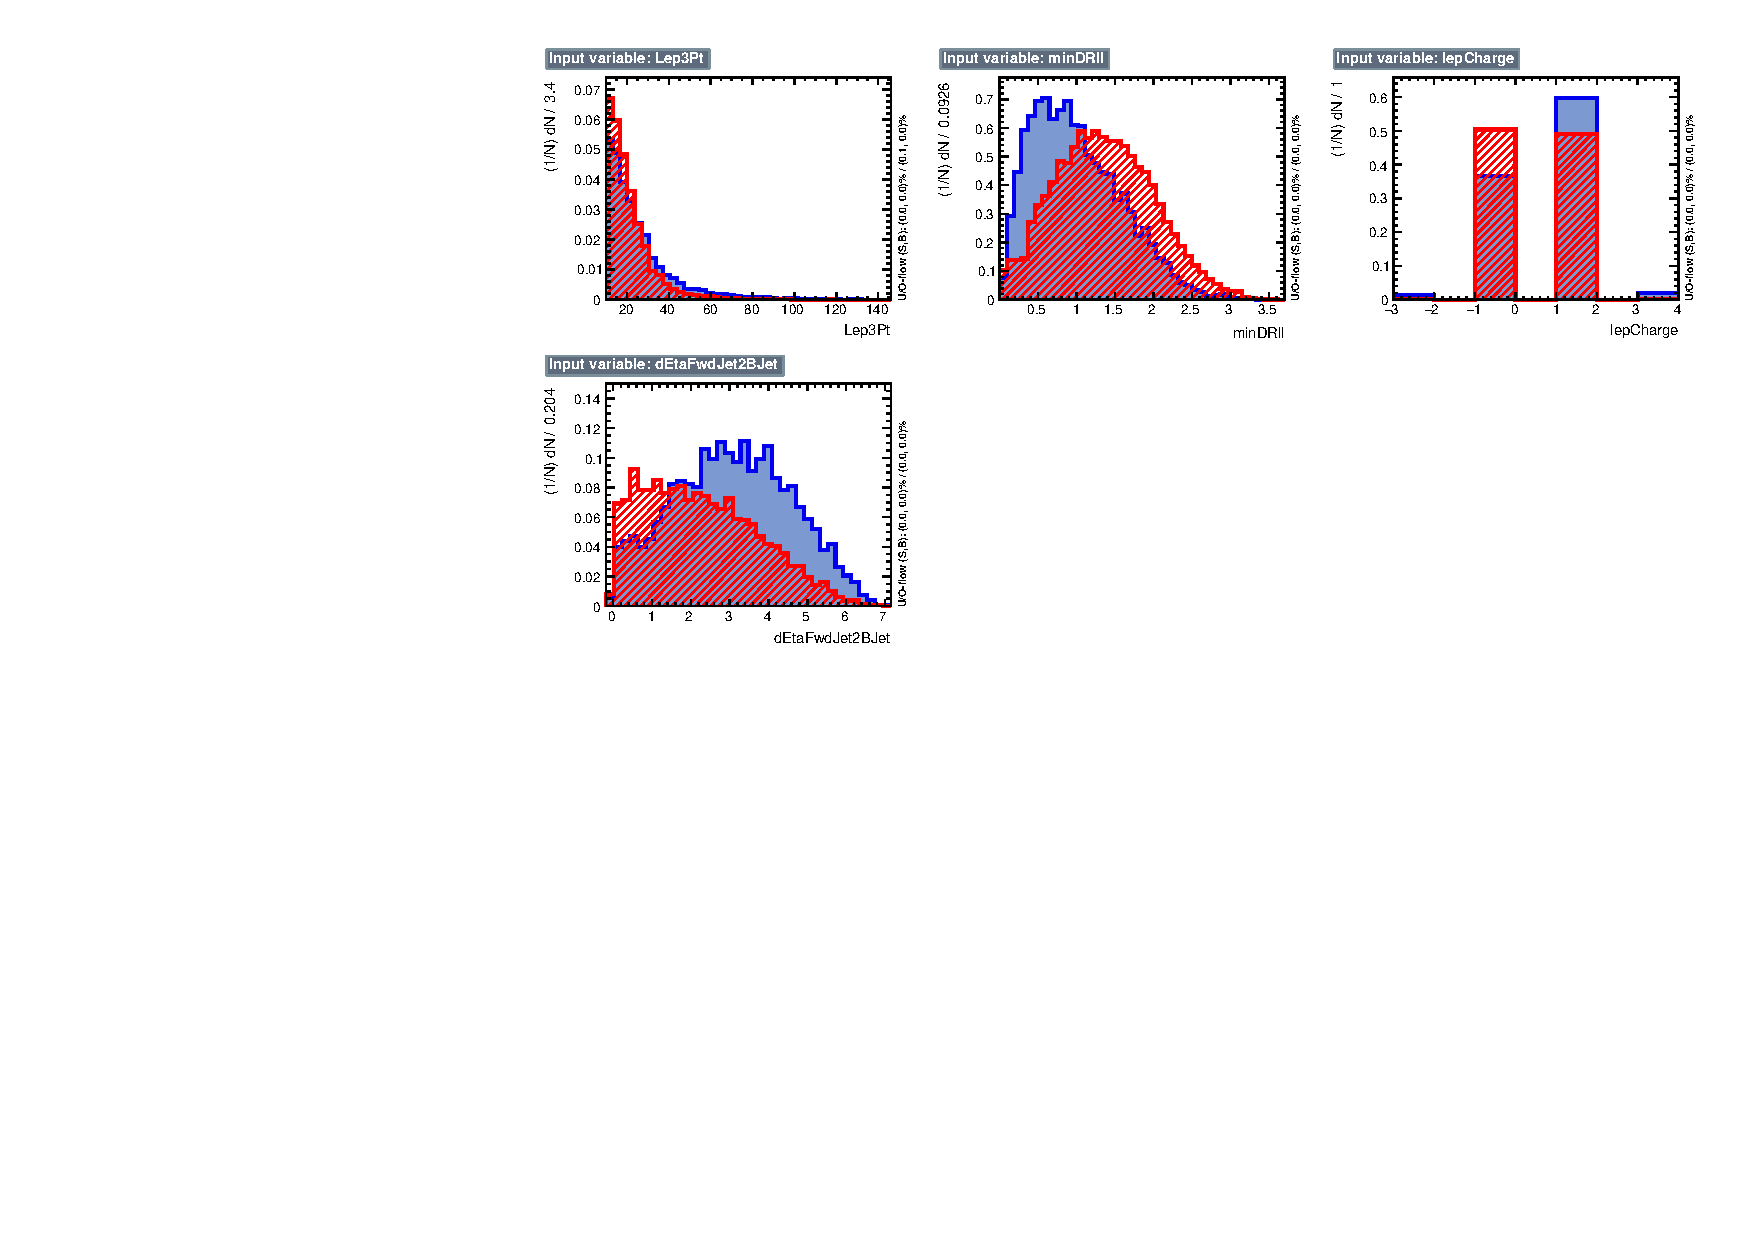
\includegraphics[width=\textwidth]{mva_input2_tt.pdf}
  \caption[BDT input variables. Discrimination against \ttbar in $3l$ channel.]{BDT input variables as seen by BDTG classifier for the $3l$ channel, \tHq signal (blue) discriminated against \ttbar\ background (red\
    ).}
  \label{mva_input_tt}
\end{figure}

\begin{figure} [!h]
  \centering
  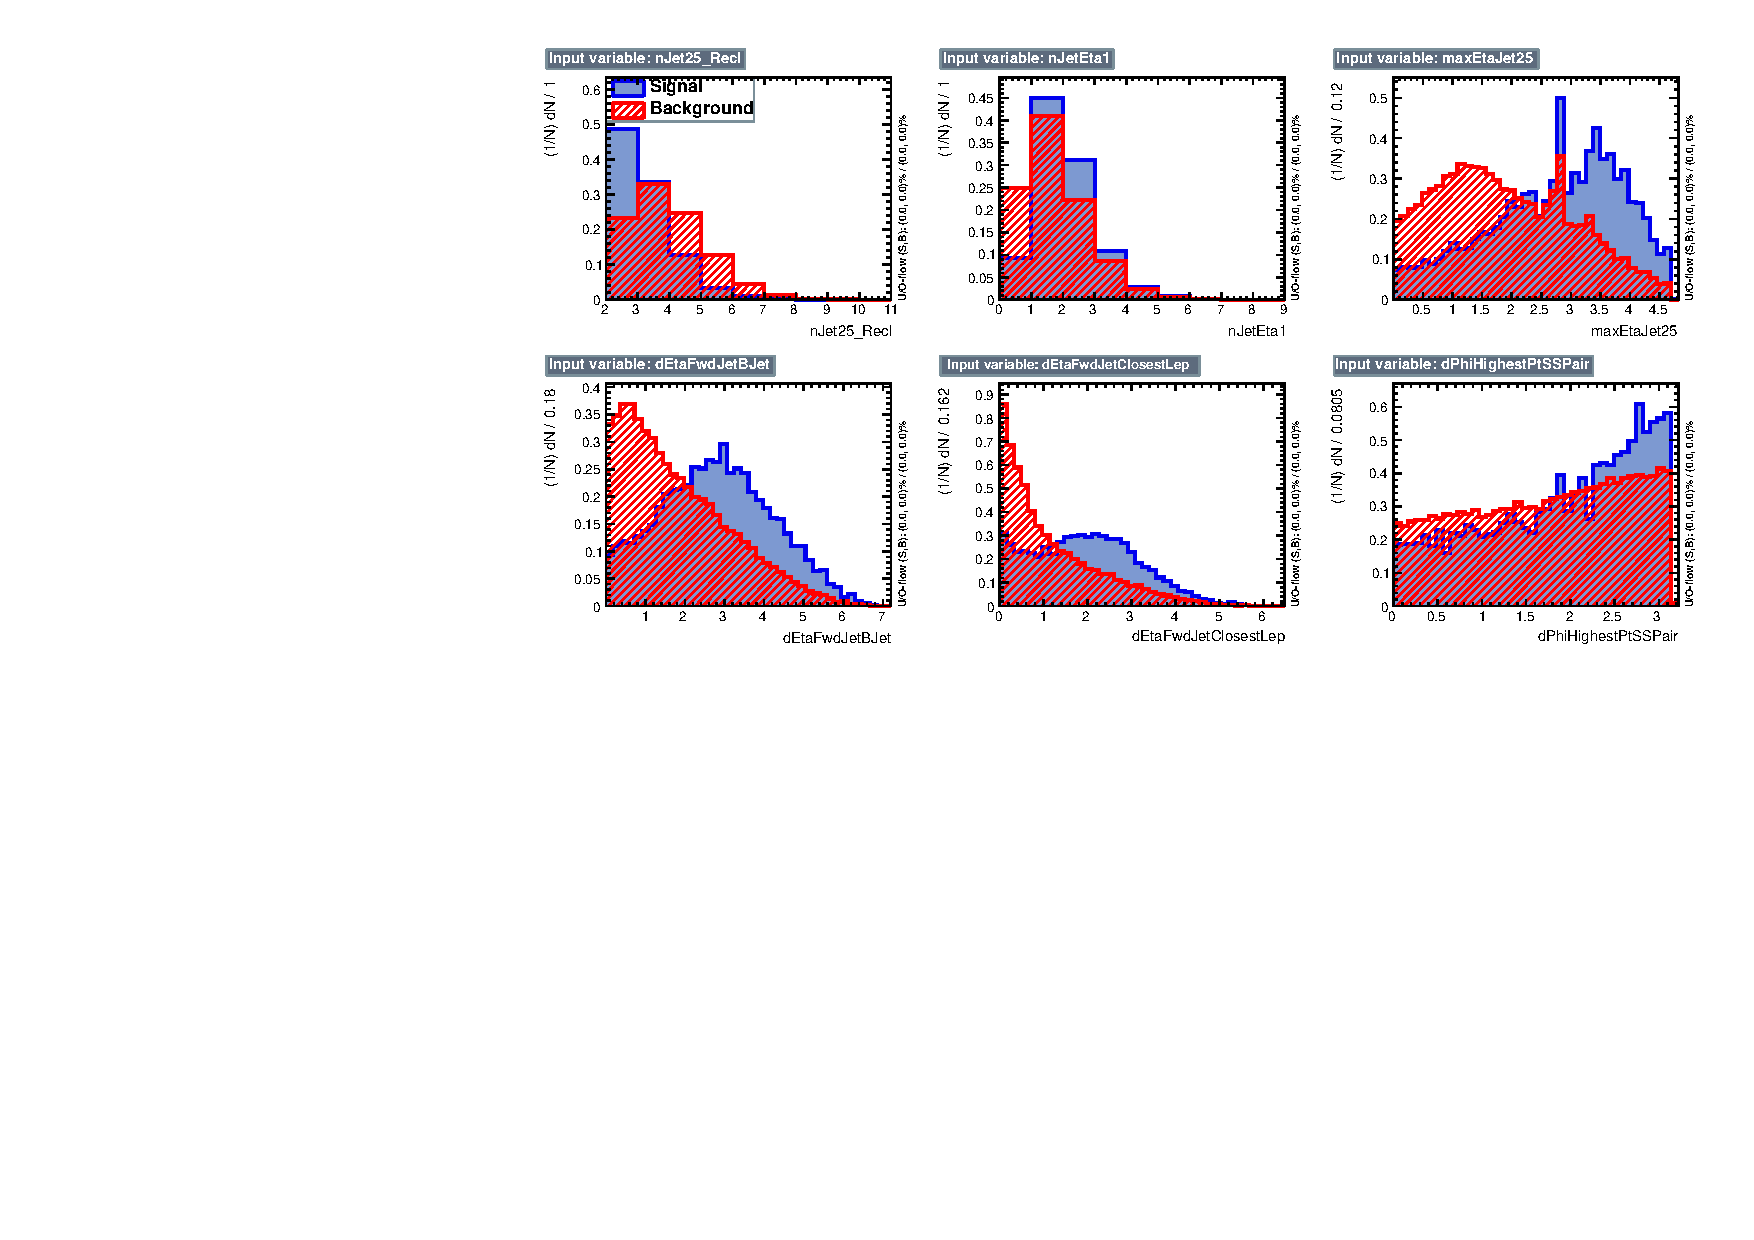
\includegraphics[width=\textwidth]{mva_input1_ttv.pdf}
  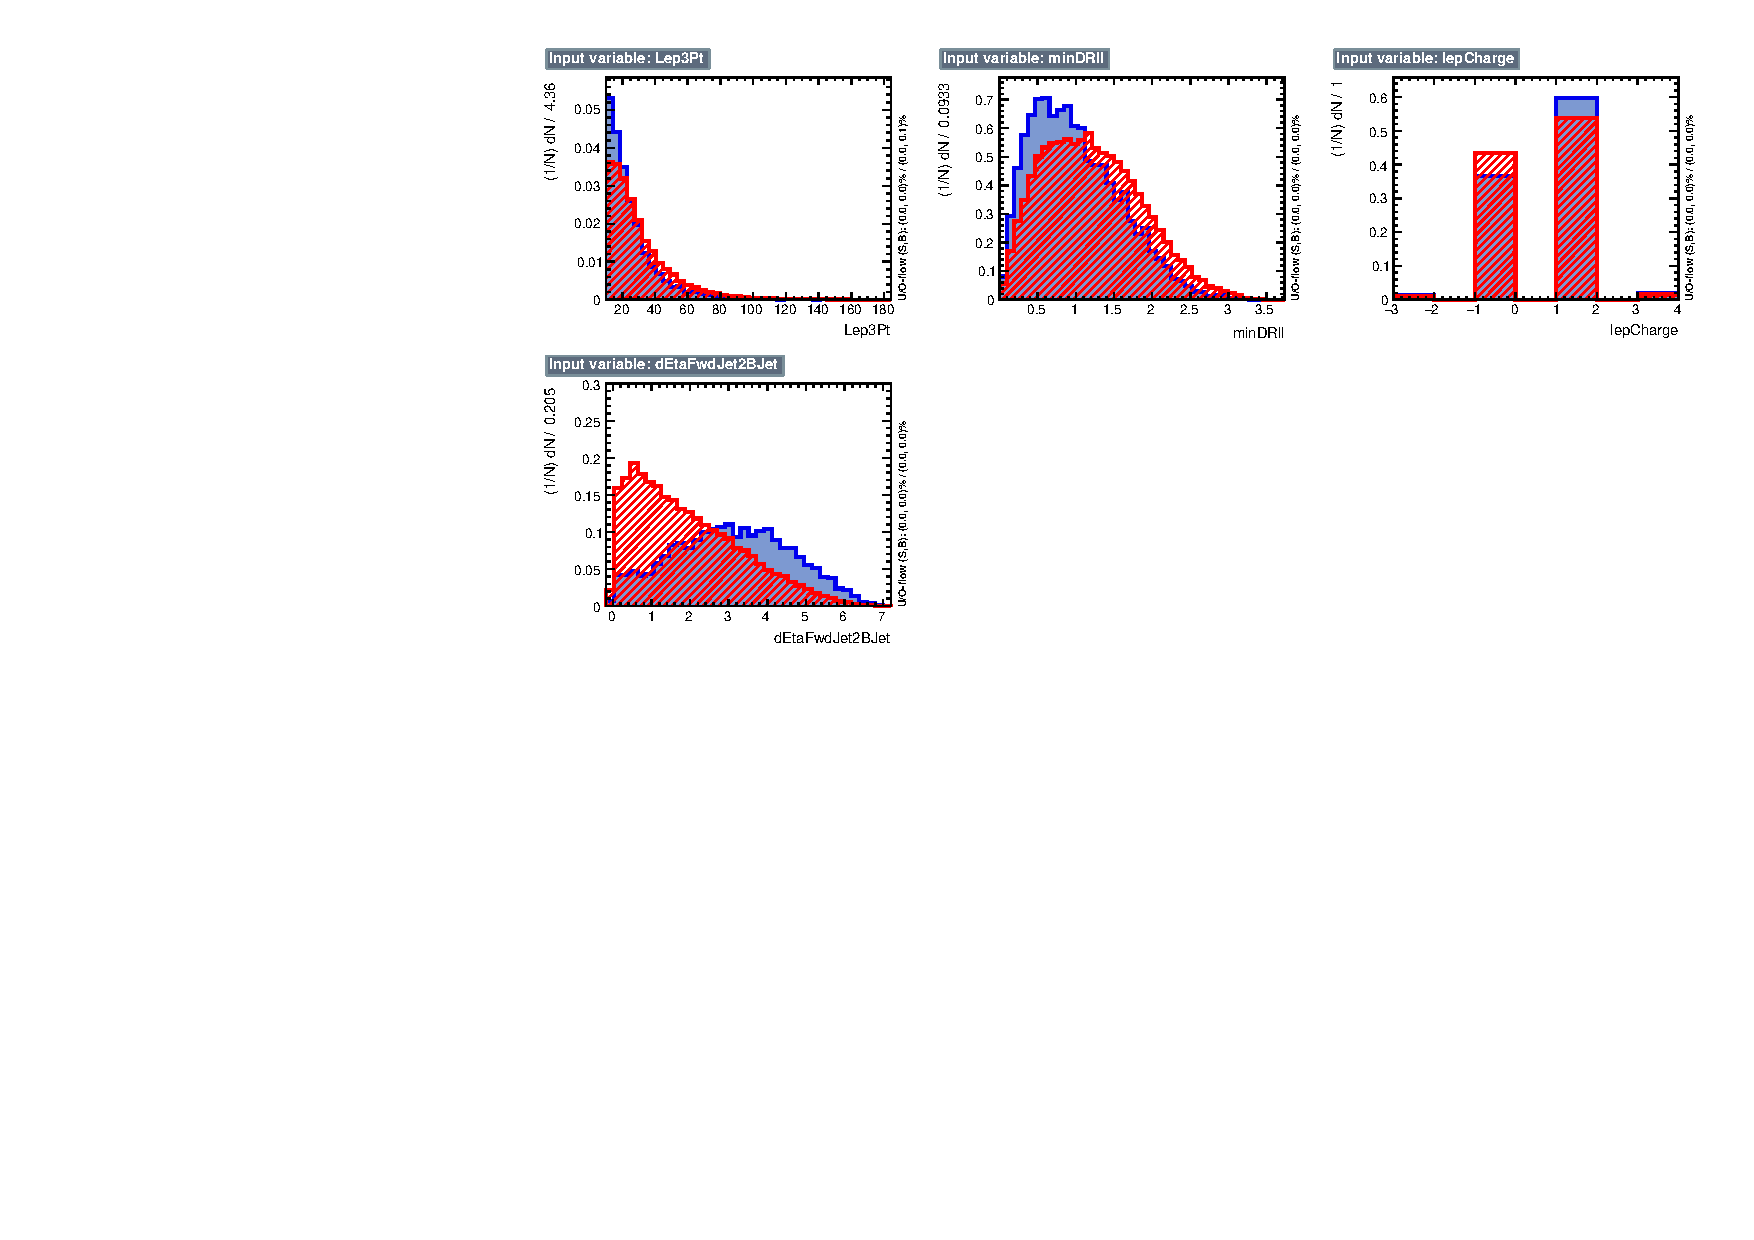
\includegraphics[width=\textwidth]{mva_input2_ttv.pdf}
  \caption[BDT input variables. Discrimination against \ttV\ in $3l$ channel.]{BDT input variables as seen by BDTG classifier for the $3l$ channel, \tHq signal (blue) discriminated against \ttV\ background (red).}\

  \label{mva_input_ttv}
\end{figure}

\newpage
\section{Pre-selection kinematic variables} \label{app:presel_plots}


